% Transfer Report: Literature Review
% Author: Andrew Hughes

\chapter{Literature Review}
\label{literaturereview}

Concurrency is an inherent part of the real world.  Multiple events
take place simultaneously, and each of these events can interact and
affect others.  Early computational models, however, take a simpler
idealised view, where events occur sequentially and in isolation.
Universal Turing machines \cite{turing:36} have proven to be
computationally complete; they are capable of simulating all recursive
functions.  However, they do not directly model concurrent execution.

So, if these models can have this level of computational power without
attempting to represent this particular aspect, why is it necessary to model
concurrency at all?  Even though a method of modelling phenomena exists,
and has a certain level of expressivity, it doesn't imply that it is the
most appropriate for a particular context.  The existence of both Turing
machines and the $\lambda$ calculus already demonstrates this point.  While
both have proven equivalent in power, they take different approaches to
achieving this.

To see the effect of concurrency on computation, consider a simple
prototypical example, as demonstrated by Milner \cite{milner:lecture}.
Observe the following programs,

\begin{align*}
\mathtt{x} & \mathtt{= 2;}\tag{P1} \\
\\
\mathtt{x} & \mathtt{= 1;}\notag \\
\mathtt{x} & \mathtt{= x + 1;}\tag{P2}
\end{align*}

\noindent where we assume that each line is an atomic action.

In a sequential system, such as may be modelled by a Turing machine or the
$\lambda$ calculus, both these programs set \texttt{x} to 2.  In such a
system, there is only a single flow of control, so nothing else can
modify the value of \texttt{x}.

However, in a concurrent system, multiple control flows or processes
exist, each running in parallel with the others.  With P1, the value
of \texttt{x} will always be equal to two immediately after execution,
as the assignment takes place within a single atomic action.  However,
in P2, another process is free to modify \texttt{x} in the
gap\footnote{Assuming \texttt{x} is accessible by more than one
  process.} between the assignment of the value 1 and the later
summation which makes \texttt{x} 2.

Thus, if P2 is run in parallel with a third program,

\begin{equation}
\mathtt{x = 3;} \tag{P3}
\end{equation}

\noindent then \texttt{x} may end up being either 2, 3 or 4, depending
on whether P3 executes before the first line, after the completion of
P2, or after the first line respectively.  With P1 and P3, only 2 or 3
can result (which one depends on the order the two programs are run).
This is known as a \emph{race condition}, as the final value of
\texttt{x} depends on the timing of the various modifications of its
value by the two programs.  The solution to this problem is to require
each program to obtain exclusive access to \texttt{x} (a lock) for the
extent of its use.

This example demonstrates that modelling concurrency is not so much
about multiple programs executing at the same time, but instead
concerns how they interact.  If each program exists in its own
isolated environment, then no interactions will take place and a
sequential model for each would be suitable.  Indeed, this is the way
most operating systems handle running multiple programs.  Thus, it
follows that sequential models are not distinct from concurrent
models, but a subset where this additional restriction of isolation
applies.

Dijkstra's classic `Dining Philosophers' problem
\cite{dijkstra:philosophers} illustrates further issues which may
arise in a situation where multiple processes must interact to achieve
their goal.  In this scenario, five philosophers are seated around a
table, each with a plate of spaghetti and a fork.  The philosophers
divide their time between thinking and eating.  In order to eat, a
philosopher must obtain two forks, necessitating some form of
interaction.  This is a common situation in concurrency, where
multiple parallel processes (the philosophers) need to gain access to
a limited resource (the forks).

In cases where things go awry, \emph{deadlock} or \emph{starvation} may
result.  For example, if the philosophers simultaneously pick up the
forks on their left, then none of them will be able to eat; they will all
end up waiting on a fork held by another philosopher.  The system is
said to be \emph{deadlocked}, as none of the processes can obtain a lock
on the resource it needs, as a lock is already held by one of the other
processes\footnote{The solution to breaking this deadlock is to break
the symmetry; if the fifth philosopher tries to take the fork on the
right first, he or she will be unable to proceed, but the first philosopher
will, using the fifth philosopher's left fork.}.  Alternatively,
\emph{starvation} may result if one of the philosophers never stops
eating and consequently never releases the forks; the resources are
unfairly distributed to the deficit of one of the processes.

As can be seen from these examples, concurrency raises issues outside
the reach of traditional sequential models of computation.  Thus, just
as there is a requirement for models of sequential computation, models
that can represent these phenomena are also necessary.  This is even
more relevant today, as hardware advances make more machines capable
of true concurrency (via dual-core processors and beyond) and
distributed computing paradigms, such as services, become more
prevalent.  To adequately work with these systems, appropriate formal
models are needed to represent them and highlight their flaws.  Many
such models have been developed, and we will now consider a subset of
these.

\section{Algebraic Process Calculi}

Algebraic process calculi model the interaction of concurrent
processes using a (usually small) set of algebraic operators, as
opposed to the true concurrency of Mazurkiewicz trace theory
\cite{maz:trace} or the graphical style associated with Petri nets
\cite{petri:phd} and Hewitt's Actor model \cite{hewitt:actor}.
Interaction between processes is via message-passing, rather than via
shared memory\footnote{Although shared memory and message-passing are
  not orthogonal; a shared memory space may be represented as a
  communicating resource in a message-passing system, while message
  queues can be implemented in shared memory.} or a tuple space
\cite{linda}.

The foundational calculi in this field are Hoare's CSP \cite{hoare:csp78},
Milner's CCS \cite{milner:ccs} and Bergstra and Klop's ACP \cite{acp}, all of
which were first developed in the late 1970s to early 1980s.  CSP was
originally developed as a programming language, with a relatively large
syntax, and later given a theoretical basis, following Milner's work on
CCS.  Both calculi have influenced each other, while starting out from
different perspectives (Milner's being more of a theoretical one).  ACP
shares many of the ideas of CCS, and can be regarded as an
`alternative formulation' \cite{acp}, using a similar set of operators
to achieve a different goal.

Here, the focus is on CCS, as it forms the basis for most of the other
calculi considered, including the $\pi$ calculus
\cite{picalctutorial} and CaSE \cite{CaSE}.  Of the three, CCS has the
most minimal syntax with additional features such as failure
(represented in both CSP and ACP) needing to be derived from or appended to
this core set.  From a theoretical perspective, this is advantageous, as
it makes reasoning over the calculus a simpler process, and, as will be
seen, adding further syntax to represent more features is a relatively
simple process.

\subsection{CCS}
\label{ccs}

In CCS, processes are modelled as terms ranged over by $E, F$.  These
process terms have the following syntax:

\begin{equation}
\label{ccssyntax}
  E, F\ ::=\ 
  0\ |\ 
  \alpha.E\ |\ 
  E\backslash\ a\ |\ 
  E\ +\ F\ |\ 
  (E\ |\ F)\ |\ 
  X\ |\ 
  \mu X.E\ |\ 
  E[f] 
\end{equation}

\noindent where $\alpha$, $a$ and $f$ are explained below.

Communication between processes is via the sending and receiving of
signals.  The internal behaviour of the processes is abstracted,
represented simply by the silent action $\tau$.  The full set of
actions, $Act = \mathcal{N} \cup \overline{\mathcal{N}} \cup
\{\tau\}$, is used to describe the behaviour of the concurrent system,
where $\mathcal{N}$ is an infinite set of names, and
$\overline{\mathcal{N}}$ is the corresponding set of co-names,
$\{\overline{a} | a \in \mathcal{N}\}$.  These names are usually used
to represent \emph{channels}, which the processes use to communicate.
Thus, $a.E$, where $a \in \mathcal{N}$, represents a process whose
first action is an input on the channel $a$, whereas $\overline{a}.E$
(where $\overline{a} \in \overline{\mathcal{N}}$) represents a process
which initially outputs on $a$.

The behaviour of a single process is thus defined as a sequence of
inputs, outputs and silent actions. This can be seen in the above
grammar, where $0$ represents the empty process, which exhibits no
behaviour, and $\alpha.E$ is the action prefix used for the limited
sequential composition of actions, where $\alpha \in Act$.

For communication to actually take place, two processes must
\emph{synchronize}; they must emit corresponding actions on the same
channel at the same time.  For this to occur, the two processes must be
running in parallel.  Parallel composition in CCS is represented by the
$|$ operator.  When two processes are composed in this way, they may
both perform their corresponding input and output actions
simultaneously, resulting in a $\tau$ action being emitted.

For instance, if $E$ is considered to be $a.0$ and $F$ to be
$\overline{a}.0$, then the process formed by the composition of these
two processes, $E|F$ may initially perform one of three actions, $a$,
$\overline{a}$ or $\tau$, to give three possible derivations:

\begin{enumerate}
\item $E\ |\ F \derives{a} 0|F$
\item $E\ |\ F \derives{\overline{a}} E|0$
\item $E\ |\ F \derives{\tau} 0|0$
\end{enumerate}

\begin{figure}  
  \centering
\[
\xy
(20,0)*{a.\nil \mid \overline{a}.\nil}="1";
(0,-15)*{a.\nil \mid \nil}="2";
(40,-15)*{\nil \mid \overline{a}.\nil}="3";
(20,-30)*{\nil \mid \nil}="4";
{\ar@/^2pc/^{a} "1";"3"};
{\ar@/_2pc/_{\overline{a}} "1";"2"};
{\ar@/^2pc/^{\overline{a}} "3";"4"};
{\ar@/_2pc/_{a} "2";"4"};
{\ar^{\tau} "1";"4"};
\endxy
\]
%  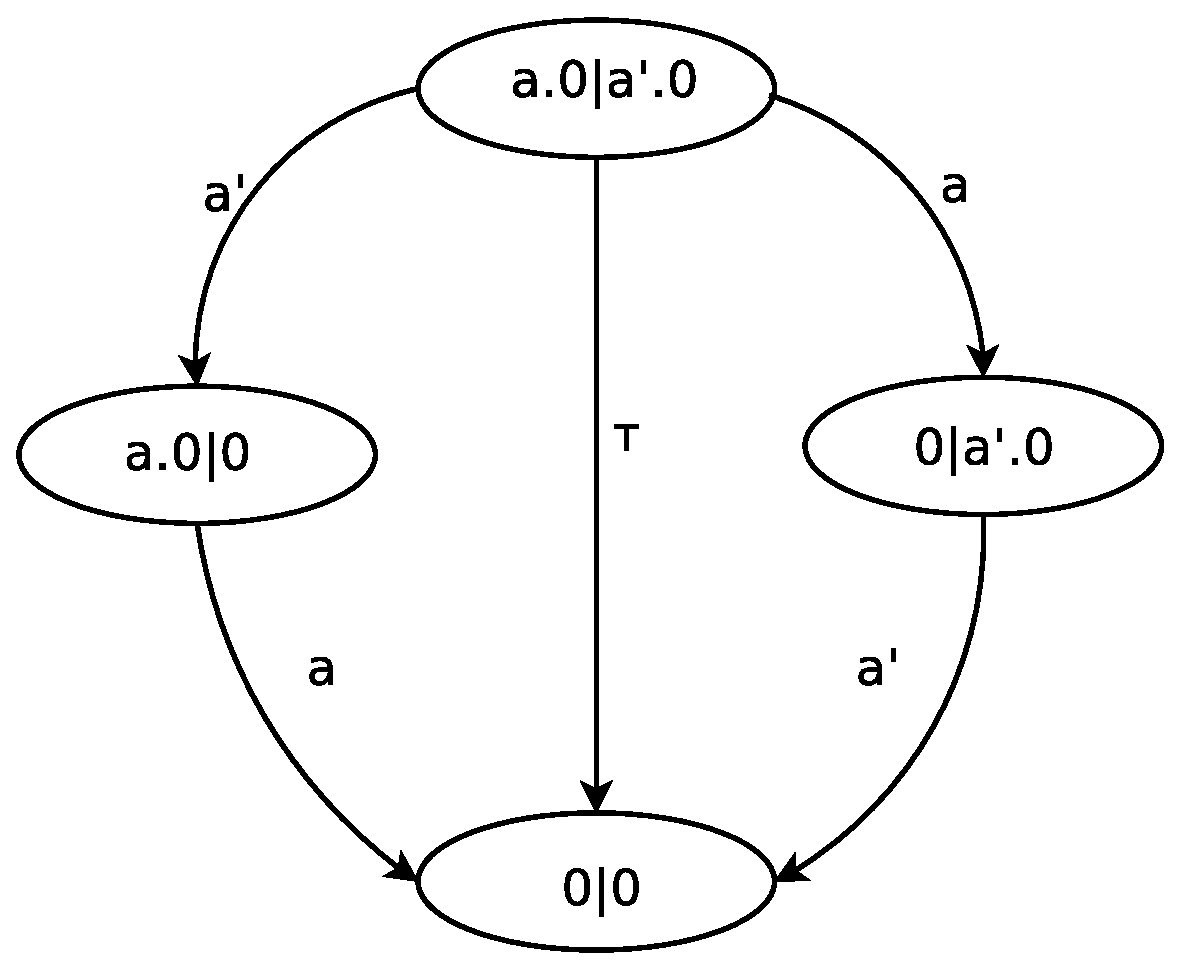
\includegraphics[scale=0.5]{graph1}
  \caption{Graph of $a.0 \mid \overline{a}.0$}
  \label{fig:graph1}
\end{figure}

This is illustrated in Fig. \ref{fig:graph1}.  To make the derivation
of $E|F$ deterministic, the scope of $a$ can be restricted.  In CCS,
an input or output can be paired with any corresponding action which
is within the scope of the channel.  To force the input of $E$ to be
paired with the output of $F$, the scope of $a$ must be restricted so
as to only include the two processes, $E$ and $F$.  This is handled by
another operator in the core syntax, $\backslash$.  The right operand
of this is the name of a channel whose scope is restricted to that of
the left operand.  In this case, $(E|F)\backslash a$ appropriately
limits the possible derivations to just $\derives{\tau}$.

The remaining binary CCS operator is $+$, which provides
non-deterministic choice between two processes.  Once a derivation is
made from one process, the option of performing the actions of the
other is lost.  This contrasts with the parallel composition operator,
where the other process remains running in parallel.  Choice thus
effectively corresponds to the familiar idea of branching found in
sequential models.  Using the same two exemplar processes again, $E +
F$ may derive as follows:

\begin{enumerate}
\item $E\ +\ F \derives{a} 0$
\item $E\ +\ F \derives{\overline{a}} 0$
\end{enumerate}


\begin{figure}  
  \centering
\[
\xy
(20,0)*{a.\nil + \overline{a}.\nil}="1";
(20,-30)*{\nil}="2";
{\ar@/^2pc/^{a} "1";"2"};
{\ar@/_2pc/_{\overline{a}} "1";"2"};
\endxy
\]
%  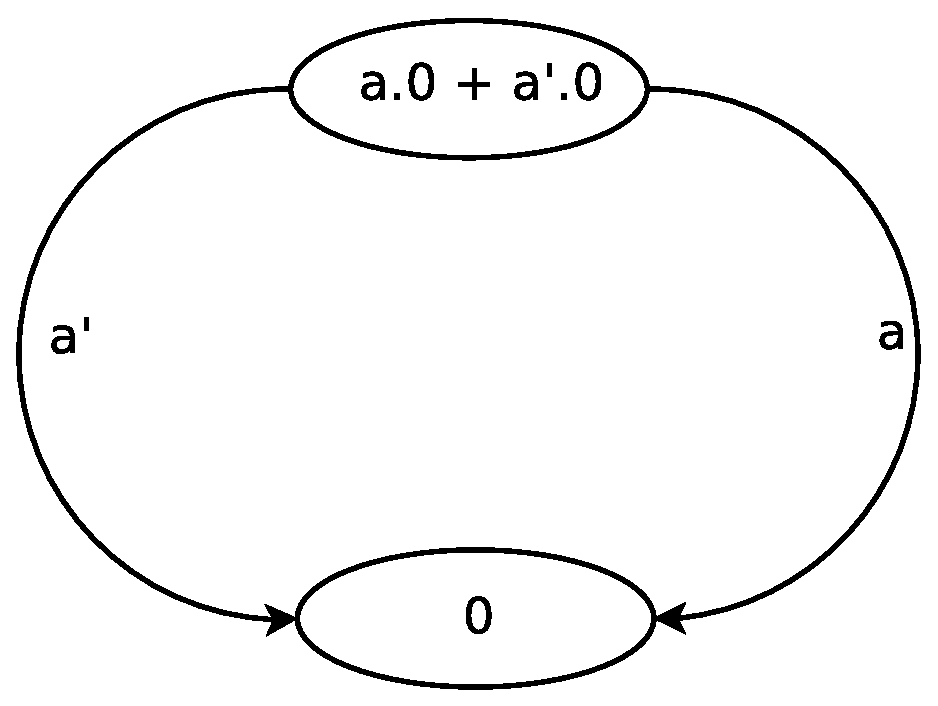
\includegraphics[scale=0.5]{graph2}
  \caption{Graph of $a.0 + \overline{a}.0$}
  \label{fig:graph2}
\end{figure}

Again, this is illustrated in Fig. \ref{fig:graph2}.  There are clearly
similarities between the two sets of possible derivations, but note
that, with choice, there is no possibility of synchronisation.

The remaining operators in CCS handle recursion and relabelling.  $\mu
X.E$ binds X with the value of $E$, so that later occurrences of $X$ are
replaced with $E$.  The function, $f$, in $E[f]$ has the type $Act
\rightarrow Act$ and converts actions, while preserving $\tau$ and
complementation.

\subsection{The Dining Philosophers in CCS}

To fully appreciate CCS, it is necessary to see how it may be used to
model an example scenario.  Consider the dining philosopher's example
illustrated above. Modelling this in CCS involves first ascertaining
what processes form the basis of this `system'.  Clearly, each
philosopher plays a part, so they should be represented by a process.
Returning to the original definition of the problem, each philosopher
may choose to eat or think.  In CCS, this can be represented as:

\begin{equation}
Philosopher = EatingPhilosopher\ +\ ThinkingPhilosopher
\end{equation}

\noindent where the philosopher is recursively defined as making the
choice between becoming an $EatingPhilosopher$ process or a
$ThinkingPhilosopher$ process.  Defining the latter is simple; 
thinking is simply some internal process of the philosopher:

\begin{equation}
ThinkingPhilosopher = \tau .Philosopher
\end{equation}

The focus of the model is on the eating process, which requires
access to the system's shared resource: the forks.  Modelling this
necessitates defining a protocol whereby the philosopher may interact
with the resource in order to obtain access to it.  From this, it
follows that the forks must also be represented as processes:

\begin{equation}
Fork = \mu X.takeFork.putDownFork.X
\end{equation}

\noindent with two communication channels, $takeFork$ and
$putDownFork$.  The fork begins its life on the table from which it
may be taken, represented here by the receipt of an input on the
$takeFork$ channel.  Once this has occurred, the process becomes
$Fork^\prime$,

\begin{equation}
Fork^\prime = putDownFork.X
\end{equation}

\noindent which represents the state where the fork is in use by a
philosopher.  The fork can't be used again until it has received an
input on $putDownFork$, which causes $X$ to be expanded and the fork to
wait for input on $takeFork$ again.

This interaction is further clarified by defining the final process,
the $EatingPhilosopher$:

\begin{equation}
EatingPhilosopher = \overline{takeFork}.\overline{takeFork}.\tau.\overline{putDownFork}.\overline{putDownFork}.Philosopher
\end{equation}

\noindent which needs to synchronize with two available $Fork$
processes to be able to eat (represented by $\tau$) and then release
the forks.  The system as a whole is modelled by running a number of
philosophers and forks in parallel (i.e. multiple copies of
Fig. \ref{fig:dpccs}), and restricting the scope of the fork channels
in order to enforce synchronisation.

\begin{figure}  
  \centering
  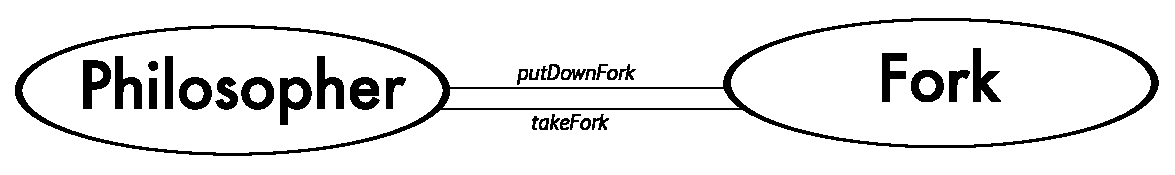
\includegraphics[scale=0.5]{philosophers}
  \caption{The Dining Philosophers in CCS}
  \label{fig:dpccs}
\end{figure}

Note that this CCS representation of the problem only models the
narrative version of the problem above.  There is no attempt to
resolve any of the competition problems, and a strong element of
non-determinism, as to which philosopher gets which fork, still
exists.  It does, however, give a formal representation of the problem
and allows the effects of varying the relative numbers of philosophers
and forks to be observed via execution of the model.

Modifying this slightly gives a model that corresponds
exactly to a specified number of philosophers and forks, $n$.  From
the definitions above, multiple variants may be generated, such that
each philosopher and fork process has a unique subscript.  For
example, $Philosopher$ becomes $Philosopher_i$, where $i = 1\dots n$.
The same subscripting also applies to the $takeFork$ and $putDownFork$
channels, so that they now correspond to a specific fork.  The
original solution can thus be represented, as the case where each
philosopher, $i$, initially performs the action $takeFork_i$ (to take
the left fork) and then $takeFork_{i-1}$ (with the exception that when
$i-1 = 0$, we use $n$) \footnote{Again, it is necessary to reverse the
  actions of $Philosopher_n$ in order to obtain a solution that does not
  deadlock.}.

This model restricts which fork is taken by which philosopher
(limiting the possible actions, and thus removing some
non-determinism), but is still prone to the effects of
non-deterministic choice (some philosophers may arbitrarily choose to
think instead) and fairness, with regards to action performance (if
the actions are performed in a depth-first manner, only one
philosopher may end up eating).  These may be regarded as
implementational aspects of the model; all these phenomena could be
represented, but a choice between these is not made at this level of
abstraction.

\subsection{Advantages and Limitations of CCS}
\label{ccslimit}

From its syntax, it is clear that CCS can model sequential behaviour
using sequential composition ($\alpha.E$), non-deterministic choice
($+$) and $\nil$.  This further confirms the intuition noted earlier that
sequential programs are a subset of the larger set of concurrent
programs.  This is illustrated by the $+$ operator, which
returns a smaller set of possible derivations, from the same initial
pair of processes, when compared with parallel composition ($|$).
These sequential operators can also be used to convert a set of
parallel-composed processes into their equivalent interleavings.

CCS can model both sequential and concurrent programs, while still
maintaining a minimal syntax.  However, the calculus is not
Turing-complete\footnote{A finite axiomatisation can be defined, if
  the simultaneous presence of parallel composition and recursion is
  avoided \cite{milner:ccsaxiom}.}; there are limitations as to what
may be expressed.  As discussed earlier, Turing completeness does not
necessarily guarantee the suitability of a model for a particular
task. Likewise, the lack of such completeness doesn't imply that the
model is unsuitable.  As shown above, an appropriate model of the
Dining Philosophers problem may be defined, without Turing
completeness.  The lack of this in CCS is not necessarily a problem.
It may even be an advantage in some cases, where this lack of
expressivity simplifies the formal reasoning over the model.

One fairly obvious limitation, and one that is relevant when
discussing Turing completeness, is that there is no data in the model.
The processes discussed so far don't explicitly communicate anything
when they send or receive signals.  Instead, behaviour arises purely
from synchronisation.  It is possible to extend CCS to represent this
by adding the concept of value passing between processes.  A host of
other process calculi have been based on such a variant of CCS, and we
will consider this in more detail as part of section \ref{mobility}.

CCS models are also relatively static; while processes may evolve
(e.g. $a.P$ may become $P$) and the number of processes in the system
may change (e.g. a process may branch using parallel composition), the
communication structure doesn't.  Notably, if a process, $E$ knows
about the channels $x$ and $y$ initially, while $F$ only knows about
$x$ (due to restriction on $y$), this status can not change during the
course of the various transitions inherent in the system.

The effect of restriction is more generally known as \emph{scoping}
and occurs frequently with reference to variables in programming
languages.  CCS doesn't allow dynamic changes to the scoping of
channels.  Instead, scoping is fixed to the static arrangement
provided by the initial system, prior to any transitions.  The
addition of dynamic scoping, often referred to as mobility, is the
major contribution of the $\pi$ calculus, a language based on CCS
covered in \ref{scopemobility}.

To conclude, there is another limitation of CCS which is less to do
with a particular concept being absent from the language, instead
being more related to its central aspect: \textbf{synchronisation}.
The problem here lies in the \emph{compositionality} of processes.
While the structure of a CCS system remains compositional, because the
result of parallel composition is determined by the behaviour of the
composed processes together with the rules of the $|$ operator, this
is not true of the synchronisation of multiple processes.

Consider the idea of broadcasting a signal to an arbitrary number of
processes.  Ideally, a general \emph{broadcast agent} should be
defined which provides this behaviour.  In CCS, there are at least two
possible ways of defining semantics for the agent, but not one that
provides a suitably compositional solution.  Perhaps the most obvious
of these is simply to extend the familiar synchronisation of two
processes.  An input and output pair can synchronize, so why not just
create multiple pairs, one for each receiving process?  For example,
transmitting a signal to two processes can be written simply as

\begin{equation}
\mathbf{\overline{a}_1.\overline{a}_2.0}\ |\ a_1.P\ |\ a_2.Q
\end{equation}

\noindent where the process on the left (in bold) forms the semantics
for the broadcast agent and the processes, $P$ and $Q$ are the
continuations of the input processes

This will work, but what happens when the broadcast agent needs to
transmit the signal to three processes?

\begin{equation}
\mathbf{\overline{a}_1.\overline{a}_2.\overline{a}_3.0}\ |\ a_1.P\ |\ a_2.Q\ |\ a_3.R
\end{equation}

\noindent The semantics of the broadcast agent have to change.  Simply
composing the third input will lead to one of the three being ignored
by the original definition of the broadcaster given above.  So, simply
enumerating multiple synchronisation pairs is not sufficient to
provide a compositional broadcast agent.

A second solution lies in recursion.  If the problem with the previous
solution lies in the broadcasting agent doing too little (i.e. not
transmitting to all the possible receivers), then, by making it
recurse, it will keep sending the output to whoever will synchronize
with it.  Thus, the example for three inputs above becomes

\begin{equation}
\mu X.\overline{o}.X\ |\ o.P\ |\ o.Q\ |\ o.R
\end{equation}

\noindent which works, and will continue to do so if a further
input process is parallel composed.  

But there is still a problem for much the same reasons as the first
solution.  This works fine on this small scale, but what happens when
this agent is placed in the context of a larger system?  Once the agent
starts its cycle of outputs, it won't stop as there exists
no base case for this recursion\footnote{A base case may be introduced
using non-deterministic choice, but there is no guarantee when this will
be invoked, if ever.}.  An output on $o$ will always be available (within
the scope of any restriction placed on that particular channel) and
the broadcasting process can never do anything else.  The result is a
constantly cycling process, which, in an implementation of this model,
would continue to consume resources.

The true solution to this problem is to enable some form of
\emph{global synchronisation}.  This requires a separate entity,
disparate from the processes involved in the communication, which can
be used to co-ordinate the synchronisation.  In the next section, a
branch of process calculi is considered which provides just such a facility.

\section{Timed Calculi}
\label{timing}

Initially, the use of the word `timed', within the context of the
calculi considered here, is a bit of a misnomer.  The notion of `time'
is generally associated with concrete real values, in units such as
minutes and seconds.  Real-time process calculi, such as those
described in \cite{aceto:timing, beaten:timing, brics:lee, lee:realtime, tccs, satoh:phd, satoh:distrib}, attempt to model this.
Instead, this section focuses on a series of discrete timed calculi
which focus on abstract time and the use of \emph{clocks} for the
primary purpose of global synchronisation (as described above).

Hennessy's Temporal Process Language (TPL) \cite{hennessy:tpl} extends
the CCS language discussed above with a single clock, akin to a
hardware clock which emits a signal at an arbitrary point in time.
These signal emissions are controlled by a concept known as
\emph{maximal progress}, which allows each process to make as much
progress as possible before the clock ticks.  Formally, this means
that all silent actions ($\tau$s) are performed before a $\sigma$
action (which represents the clock signal) occurs.

This is of little use unless the actions of the processes can actually
depend on the behaviour of the clock.  The two are related via the
addition of a timeout operator.  This takes the form

\begin{equation}
\timeout{E}{\sigma}{F}
\end{equation}

\noindent where $E$ and $F$ are processes and $\sigma$ is the clock.  In
short, $F$ acts if $E$ \emph{times out} on the clock, $\sigma$.  This is
similar to non-deterministic choice, in that only one of the two
processes will ever act and the behaviour of the other is lost.  Here,
however, the choice is determined by the clock (and thus effectively by
the other processes, as it is their behaviour which controls when the
clock will tick).

With these additions, the problem of defining a suitable compositional
broadcast agent, as mentioned above, can be solved.  Recall the second
solution, which used recursion.  Now, with the addition of an external
entity (the clock) and a way of relating it to the processes involved
(timeouts), a base case may be provided via recognition of the point
when no more synchronisations may occur.  This can be added to the
earlier recursive solution

\begin{equation}
\mu X.\timeout{\overline{o}.X}{\sigma}{0}\ |\ o.P\ |\ o.Q\ |\ o.R
\end{equation}

\noindent by simply adding a timeout which stops the recursion.  This
works because the synchronisations of the input processes with the
output of the broadcast agent generate silent actions and thus invoke
maximal progress.  While there is a choice between a silent action
(due to the broadcasting agent synchronising with an input) and a
clock tick, the silent action always takes precedence and thus every
possible synchronisation occurs.  Once no more synchronisations are
possible, the clock is allowed to tick and the recursion stops.

\subsection{Extending TPL}
\label{tplext}

The extensions to TPL considered here focus on expanding the
scalability of the language.  As demonstrated above, TPL adequately
provides for situations where an arbitrary number of processes must
synchronize.  But what happens when a solution, like the one above, is
integrated into a larger system?  With only one clock, further
problems occur.  The use of the clock in one subsystem may conflict
with its use in another, and there is no clock available to
co-ordinate the subsystems themselves.

The Calculus for Synchrony and Asynchrony (CSA) \cite{csa} extends TPL
with the idea of multiple clocks, drawn from PMC\footnote{PMC also
  differs from TPL in its use of \emph{insistent} actions; all must be
  performed before a clock tick.}\cite{pmc}. However, while having
multiple clocks allows the use of differing patterns of
synchronisation, it increases the number of clock ticks present within
the system.  With five clocks, even the nil process has five possible
transitions (as clocks idle over nil).

CSA solves this to a limited extent by localising maximal progress to
a pre-defined scope for each clock.  A more elegant solution is
provided in the Calculus for Synchrony and Encapsulation (CaSE)
\cite{CaSE}, which introduces a clock hiding operator into the syntax.
The effect of this is the introduction of \emph{synchronous
  encapsulation}, as hidden clocks emit $\tau$ actions (as opposed to
ticks) outside the operator's scope.  This can be used, in conjunction
with restriction, to produce a hierarchy of components.  The actions
of these subsystems can be represented purely as silent actions, and,
when combined with the global form of maximal progress introduced by
TPL and retained in CaSE, integrated into the `synchronous cycle'
\cite{CaSE} of clocks at the level above.  CaSE is further discussed
in \ref{case}, where it forms the basis for the calculus of
\emph{Typed Nomadic Time} (TNT).

\subsection{Advantages and Disadvantages of Timed Calculi}
\label{timelimit}

The main advantage of the timed calculi we have discussed here is that
they allow, via the introduction of \emph{global synchronisation}, the
construction of systems on a larger scale than those that could be
created purely with CCS.  With CaSE, components can be created which
consist of multiple processes and clocks.  These can then be
successfully integrated together to form new components.

Global synchronisation allows the problem of defining a compositional
broadcast agent, cited earlier in \ref{ccslimit}, to be solved, but
these timed calculi still retain the other problems with CCS we
mentioned there.  Neither TPL, PMC, CSA nor CaSE explicitly include
data within the model.  This is not necessarily a disadvantage; it is
possible to model data implicitly, via the use of silent actions, and
including data in the model complicates formal reasoning and
equivalence theories.

More importantly, these calculi all still retain a static structure.
The scope of restriction or clock hiding doesn't change as the
processes evolve.  This prevents these calculi from being used to
model mobile systems where these elements do change, although they
are perfectly suited to modelling static dataflow-oriented systems
such as those in \cite{WICSA} and \cite{cashews-sem}.

In contrast, the following section contains a discussion of calculi
which, while lacking the scalability of the timed languages just
illustrated, can model \emph{mobile systems}.

\section{Mobility}
\label{mobility}

Within the field of algebraic process calculi, there are two clear ways
in which the dynamic nature of a system is modelled.  The most
well-known is the form of mobility present within Milner's $\pi$
calculus which allows the scope of a name to change as the system
evolves.  This concept can be thought of in a similar way to the
reference passing that occurs in most programming languages; part of the
program begins with no knowledge of an entity, and later gains knowledge
by obtaining a reference to it.

Models in the $\pi$ calculus are not really mobile in the sense of
something moving from one place to another.  This isn't possible, as
there is no real notion of `place' to begin with.  However, the addition
of this mechanism does allow the modelling of dynamic systems, such as a
mobile phone network \cite{milner:lecture}, and is sufficiently
expressive as to allow it to encode Church's $\lambda$ calculus
\cite{funcproc}.

A more naturalistic form of mobility is found in calculi which allow
entities to \emph{migrate}.  One of the primary exponents of this is
Cardelli and Gordon's ambient calculus \cite{amb}, which groups
composed processes inside \emph{ambients}.  These ambients can be
moved up and down a nested hierarchy of such objects, or destroyed.  The
calculus differs from those previously considered, in that it
lacks communication primitives.  Surprisingly, the base syntax is
sufficient to allow communication to be encoded within them, and
indeed the entire asynchronous form of the $\pi$ calculus can be
represented.

The following two sections consider examples of both types of mobile
calculi in more detail.
 
\subsection{Scope Mobility}
\label{scopemobility}

\subsubsection{The $\pi$ Calculus}
\label{picalculus}

The $\pi$ calculus follows on from Milner's earlier work on CCS
discussed in \ref{ccs}. Essentially, it is a value-passing form of CCS
with a generalisation from values and channels to simple \emph{pure
  names}.  Thus, channels can be passed between processes, as well as
values, which means that their scope may change during execution.

To make this clearer, consider the syntax of the form of $\pi$ calculus
given in \cite{funcproc}

\begin{equation}
\label{pisyntax}
  E, F\ ::=\ 
  0\ |\ 
  \overline{x}y.E\ |\ 
  x(y).E\ |\ 
  (a)E\ |\ 
  (E\ |\ F)\ |\ 
  !E
\end{equation}
  
\noindent which is a minimal version containing replication as opposed
to recursion, with $a$ a channel name and $x$ and $y$ being defined
below.  Compare this with the syntax given for CCS in Eqn.
\ref{ccssyntax}.  The nil process, $0$, is still present, as is parallel
composition and restriction (although in a new form, $(a)E$).
Non-deterministic choice is present in the original version of the $\pi$
calculus presented in \cite{picalctutorial}, but is removed from the
version given in \cite{funcproc} due to the formulation of semantics
used there.  $!E$ is the syntax for replication, which replaces
recursion in this particular variant of the calculus to give a simpler
theoretical treatment, while still doing much the same job.

The main distinction between the two lies in the remaining element of
the syntax: prefixing.  In CCS, a more general syntax, $\alpha.E$,
where $\alpha \in \mathcal{N} \cup \overline{\mathcal{N}} \cup
\{\tau\}$, is used and includes input, output and silent actions.  In
the syntax given above for the $\pi$ calculus, the input ($x(y)$) and
output ($\overline{x}y$) syntax are given separately, and the input
prefix is \emph{binding}\footnote{When an input is received on $x$,
  $y$ is bound to the value of that input, which is then substituted
  for $y$ in the continuation of that process.} like restriction. $x$
and $y$ are both names, where `$x$ [is] the \emph{subject} and $y$ the
\emph{object}' \cite{funcproc}.  Silent actions no longer appear in
prefix form, but do occur as $\tau.E$ in some variants of the $\pi$
calculus.

The distinction between the $\pi$ calculus and value-passing forms of
CCS, which also use this form of prefixing, lies in $x$ and $y$ being
drawn from the same set in the $\pi$ calculus.  In contrast,
value-passing forms of CCS keep the two sets distinct, so that the
channel and value names do not intersect.  This change is what
gives $\pi$ calculus its power, as channels can now be used as the
object of an input or output.  Thus,

\begin{equation}
x(y).\overline{y}x.0
\end{equation}

\noindent becomes perfectly valid.

This also has an effect on restriction.  Recall that, in CCS,
$(a.0|\overline{a}.0)\backslash a$ restricts the scope of $a$ to just
the two processes, $a.0$ and $\overline{a}.0$, making a synchronisation
the only possible action which may be performed.  Now consider the
following processes defined using the $\pi$ calculus:

\begin{equation}
(a)(a(x).\overline{x}a.0\;|\;\overline{a}y.0)\;|\;y(z).P
\end{equation}

\noindent where the scope of $a$ is again restricted, this time to the
two processes $a(x).\overline{x}a.0$ and $\overline{a}y.0$.  If these
two processes synchronize, the system evolves to:

\begin{equation}
(a)(\overline{y}a.0\;|\;0)\;|\;y(z).P
\end{equation}

\noindent with $x$ becoming bound to the channel name, $y$.  This shows
how the $\pi$ calculus allows channel names to be passed between
processes, but it is the next transition that is really interesting.
$\overline{y}a.0$ will pass the channel name, $a$, to $y(z).P$, which is
outside the scope of the restriction imposed on $a$.  As a result, the
scope of $a$ is \emph{extruded}:

\begin{equation}
(a)(0\;|\;0\;|\;P\{a/z\})
\end{equation}

\noindent so as to include the process, $P$, in which $a$ is now
substituted for $z$.  Further, one of the structural congruence rules of
the $\pi$ calculus \cite{funcproc}:

\begin{equation}
(x)(P\;|\;Q) \equiv P\;|\;(x)Q\text{ if x not free in P}
\end{equation}

\noindent may be used to perform \emph{scope intrusion}, giving:

\begin{equation}
0\;|\;0\;|\;(a)(P\{a/z\})
\end{equation}

\noindent as the channel $a$ no longer occurs in the other two
processes.  These changes in scope are central to the concept of
mobility within the $\pi$ calculus.  They reflect the dynamic
environment of the processes represented, and give the calculus a
greater expressivity.

\subsubsection{Variants of the $\pi$ Calculus}
\label{pivariants}

Multiple variants of the $\pi$ calculus exist, including various
evolutions of the syntax and semantics.  As noted above, replication
is only introduced in the version of the calculus given in
\cite{funcproc}, which also defines a reduction-based semantics.  The
earlier tutorial papers \cite{picalctutorial} instead use recursion
and a structured operational semantics, based on a labelled transition
system.

The polyadic $\pi$ calculus \cite{milner:93polyadic} is a more
distinct variant.  Essentially, this involves a syntactic change to
input and output, so that a tuple is used, as opposed to the single
names used in the monadic $\pi$ calculus\footnote{This is a term used
  to refer to the original $\pi$ calculus in retrospect.}.  Having
this as a core part of the syntax provides advantages in representing
abstractions and giving a natural sort discipline\footnote{Sorts are a
  way of applying typing to the $\pi$ calculus, which will be covered
  further in section \ref{typedcalculi} on typed calculi.}.  However,
it is also possible to simply provide an encoding of this in the
monadic variant.

Doing so is not simply a matter of transmitting each value in
sequence; the operation needs to respect the atomicity implicit in the
use of multiple names.  Observe the following example from
\cite{milner:93polyadic}:

\begin{equation}
x(yz)\;|\;\overline{x}y_1z_1\;|\;\overline{x}y_2z_2
\end{equation}

\noindent where the process on the left should receive either $y_1$ and
$z_1$ or $y_2$ and $z_2$.  With the following semantics,

\begin{align}
\seml x(yz) \semr & \eqdef x(y).x(z) \\
\seml \overline{x}yz \semr & \eqdef \overline{x}y.\overline{x}z
\end{align}

\noindent the two sending processes can interfere with one another.
$y$ will become bound to either $y_1$ or $y_2$ on the first
synchronisation, which is fine, but $z$ may then receive whichever of
these two remains instead of the second element in the tuple.  This
happens because there is no link between the two synchronisations.
Thus, each subsequent transmission results in a new competition
between the two processes as to who actually synchronises with the
receiver.

The solution to this problem is to make use of a \emph{private
  channel}.  Before transmitting any of the names that form part of
tuple, the sending process passes a reference to a new channel to the
receiver.  The receiver then uses this channel to receive the contents
of the tuple, rather than relying on an existing channel, which may be
prone to interference.  Thus, the semantics become:

\begin{align}
\seml x(yz) \semr & \eqdef x(w).w(y).w(z) \\
\seml \overline{x}yz \semr & \eqdef (w)(\overline{x}w.\overline{w}y.\overline{w}z)
\end{align}

\noindent where $w$ is the new private channel created to facilitate
the process of transmitting the tuple.  This ability to encode the
polyadic variant in the original monadic calculus implies that the new
syntax fails to yield any greater expressivity, but this is not really
the motivation behind this extension.  Instead, what this provides is
a more natural way of transmitting information, which makes modelling
relatively complex systems easier.

The asynchronous $\pi$ calculus \cite{boudol:asynchrony,
  honda:asynchronouscommunication, sangiorgi:asynchronousprocesscalculi}
  deliberately reduces the level of expressivity in order to simplify
  reasoning and provide a better framework for distributed
  implementations.  The output prefix, $\overline{x}y.E$ is replaced
  with $\overline{x}y.0$, so that there is no continuation after an
  output.  In the original synchronous $\pi$ calculus, the behaviour of
  the continuation, $E$, is blocked until a synchronisation with a
  recipient can occur.  This doesn't occur in the asynchronous variant,
  as there is no longer any behaviour dependent on this output
  occurring.

  Synchrony can be emulated in the asynchronous polyadic $\pi$
  calculus, just as synchronous messaging frameworks, such as TCP, can
  be implemented on top of an asynchronous network.  The receiver
  simply has to acknowledge receipt of the message by replying to the
  sender.  The following semantics are given for the monadic prefixes
  in \cite{boxedamb01}:

\begin{align}
\seml \overline{c}x.P \semr & \eqdef (r)(\overline{c}xr\;|\;r.P) \\
\seml cy.P \semr & \eqdef c(yr).(\overline{r}\;|\;P)
\end{align}

\noindent where $r$ is not free in $P$.  The output is encoded as the
transmission of a tuple containing two names: $x$, the original name
being sent, and $r$, a new channel created to receive the
acknowledgement from the recipient.  This runs in parallel with
another process that awaits an input on $r$\footnote{$r$ is a
  syntactic abbreviation for $r()$ i.e. the input is an empty tuple.}
before continuing with $P$.  Thus, the original synchronous behaviour
is emulated, as $P$ will not evolve until the receiver has obtained
the private channel, $r$, and replied.

Other changes to the calculus are also commonly adopted to reduce its
expressivity, thus making more proofs feasible.  These include:

\begin{itemize}
\item \emph{input localisation} \cite{merro:locality}, whereby a link
  received from another process can not be used for input.  For
  example, a process $a(x).P$ may not use $x$ as a channel upon which
  to receive input in $P$.
\item \emph{uniform receptiveness}
  \cite{sangiorgi:uniformreceptiveness}, where the input end of a link
  occurs only once syntactically and is replicated so as to be always
  available.
\item \emph{input-guarded replication}, which is not just restricted
  to uniform receptiveness variants, but is generally used as a more
  restricted form of replication (so the replication operator becomes
  $!a(x).P$ rather than $!P$).
\end{itemize}

The final variant of the $\pi$ calculus considered here is the
extension to higher-order operations.  The most obvious change to make
in this direction is to allow processes to be exchanged.  Such a
second-order form of the calculus is given by the \emph{Calculus of
  Higher Order Communicating Systems} (CHOCS) \cite{thomsen:chocs},
which actually predates the $\pi$ calculus itself.  This extended CCS
with mobility by allowing processes, rather than channel names, to be
transmitted.

The more general area of higher-order $\pi$ calculus, and the theory
behind it, is covered in Sangiorgi's thesis \cite{sangiorgi:phd}.  It
defines an extension to the $\pi$ calculus, HO$\pi$, which not only
allows the transmission of names (first-order) and processes
(second-order), but also parameterised processes of arbitrarily high
order ($\omega$-order).  This is best illustrated by some examples,
drawn from \cite{sangiorgi:phd}.  In the simplest case, an `executor'
process can be defined, $x(X).X$, which will receive and then execute an
arbitrary process.  Placing this in an appropriate context,

\begin{equation}
\overline{x}P.Q\;|\;x(X).X
\end{equation}

\noindent the process on the left, $\overline{x}P.Q$, will transmit
the process, $P$, to the executor before continuing as $Q$.  Thus,
following the synchronisation of the two processes, this system
evolves to become:

\begin{equation}
Q\;|\;P
\end{equation}

\noindent where the process $P$ having being substituted for $X$.  

A more complex example is given by considering Milner's encoding of
the natural numbers \cite{milner:93polyadic}.  A natural number, $n$,
is encoded as a series of outputs on $y$, the number of which is equal
to $n$ (represented as $\overline{y}^n$), followed by a transmission
on $z$ to indicate zero and thus, the end of the number:

\begin{equation}
\seml n \semr \eqdef (y,z)\overline{y}^n.\overline{z}
\end{equation}

\noindent Using HO$\pi$, the addition of these numbers can be encoded
in a very simple way.  In the $\pi$ calculus, summation is achieved
via an indirect reference to the two numbers, using channel names.  In
HO$\pi$, the parameterised processes or \emph{agents} that represent
the numbers can be used directly in the representation of addition.
Thus, actually adding the two numbers together becomes a simple matter
of running the two concurrently, and linking them via a common
channel.

A $Plus$ agent, which performs the addition of two numbers, can be
defined as follows:

\begin{equation}
Plus \eqdef (X,Y)(y,z)((x)(X\langle y,x\rangle \;|\;x.Y\langle y,z\rangle ))
\end{equation}

\noindent where both $X$ and $Y$ are agents with two parameters,
corresponding to $y$ and $z$ respectively in the definition of $\seml
n \semr$ above.  The operation of this agent is best demonstrated by
example.  Assume $X$ is two and $Y$ is three, represented in HO$\pi$ as:

\begin{align}
X(y,z) & \eqdef \overline{y}.\overline{y}.\overline{z} \\
Y(y,z) & \eqdef \overline{y}.\overline{y}.\overline{y}.\overline{z}
\end{align}

\noindent and retaining the same representation used for $\seml n
\semr$ above.  When $X$ and $Y$ are passed to the $Plus$ agent, $X$ is
instantiated with a new private channel, $x$, in place of $z$ in the
above.  $Y$ is then prefixed with an input on this same channel, so
that the $y$ outputs occurring in $Y$ only execute after those in $X$.
This leads to the following sequence of transitions:

\begin{equation}
  \lderives{y} \lderives{y} \lderives{\tau} \lderives{y} \lderives{y} \lderives{y} \lderives{z}
\end{equation}

\noindent which is close to the sequence that occurs for the
representation of five in HO$\pi$:

\begin{equation}
  \lderives{y} \lderives{y} \lderives{y} \lderives{y} \lderives{y} \lderives{z}
\end{equation}

Formally, the two are \emph{weakly bisimilar}.  A \emph{bisimulation} is
a symmetric binary relation between two processes, which exists if each
process can simulate the behaviour of the other.  $R$ is such a relation
iff, for all pairs of processes $(p,q)$ in $R$ and all actions,
$\alpha$\footnote{The bisimulation definition given here is more
applicable to the static systems of CCS.  Although it holds for this
simple example, a more detailed method of bisimulation is required to
handle the dynamic binding that occurs in the $\pi$ calculus and its
derivatives.}:

\begin{enumerate}
\item $P \derives{\alpha} P^\prime \implies \exists Q^\prime\ such\
  that\ Q \derives{\alpha} Q^\prime\ and\ (P^\prime,Q^\prime) \in R$
\item $Q \derives{\alpha} Q^\prime \implies \exists P^\prime\ such\
  that\ P \derives{\alpha} P^\prime\ and\ (P^\prime,Q^\prime) \in R$
\end{enumerate}

For a weak bisimulation, $\tau$ transitions are effectively ignored.
A series of such transitions,
$\derives{\tau}\derives{\tau}\derives{\tau}\dots$ is abbreviated to
$\obsderives{\tau}$ and $\obsderives{\tau} \derives{a}
\obsderives{\tau}$ is deemed equivalent to $\derives{a}$.  As the
additional $\tau$ transition in the $Plus$-based derivation is the
only difference between the two, the two can be deemed equivalent
under the rules of weak bisimulation.

Returning to HO$\pi$, the most interesting point about this calculus
is not that it provides the means to formulate abstractions of the
type just demonstrated, but that, in doing so, it adds no further
expressivity.  Indeed, Sangiorgi, in his thesis \cite{sangiorgi:phd}
demonstrates how a HO$\pi$ calculus can be represented in the $\pi$
calculus.  Thus, just as with the polyadic variant, the benefit of
using HO$\pi$ comes not from increased expressivity, but from the
additional ease it provides in modelling certain scenarios.

\subsubsection{The Join Calculus}
\label{join}

The Join calculus \cite{join} takes the asynchronous $\pi$ calculus as
its basis, and focuses on providing a formalism better suited as the
basis for a distributed implementation.

Take the following example of a $\pi$ calculus process given in
\cite{joinresults}:

\begin{equation}
x(y).P\;|\;x(z).Q\;|\;\overline{x}a
\end{equation}

\noindent where two processes are waiting to receive input on $x$.
The problem with implementing this in a distributed setting is that
there is no concept of location with the $\pi$ calculus.  Each of the
two receiving processes or \emph{receptors}\footnote{The join calculus
  uses an analogy with chemistry to describe its behaviour, based on
  the \emph{CHemical Abstract Machine} (CHAM) \cite{cham}.} may be
located at an arbitrary distance both from each other and from the
transmitter, $\overline{x}a$.  As a result, a \emph{distributed
  consensus problem} arises as to which of the two receptors will
receive the transmission.

The join calculus provides a solution to this problem by altering the
syntax of the $\pi$ calculus.  The asynchronous variant of the
syntax given in Eqn. \ref{pisyntax} becomes:

\begin{align}
\label{joinsyntax}
  P, Q\ & ::=\ 
  0\ |\ 
  \mathtt{def}\ D\ \mathtt{in}\ P\ |\
  (P\;|\;Q)\ |\ 
  x\langle \tilde{v} \rangle \\
  D, E\ & ::=\
  J \rhd P\ |\
  D \wedge E\ |\ 
  \mathbf{T} \\
  J,J^\prime\ & ::=\ 
  x\langle \tilde{v} \rangle\ |\
  (J\;|\;J^\prime)
\end{align}

\noindent with $\mathbf{T}$ being the empty definition and a clear
focus on linking the receptors in $D$ to the emissions occurring in $P$
(both represented by the same syntax, $x\langle \tilde{v} \rangle$).
The use of this is most clearly demonstrated by example:

\begin{equation}
  \mathtt{def}\ (x\langle y \rangle \rhd P) \wedge (x\langle z \rangle \rhd Q)\ \mathtt{in}\ x \langle a \rangle
\end{equation}

\noindent which has essentially the same behaviour as the $\pi$
calculus example presented earlier.  $x\langle y \rangle \rhd P$
receives an input, $y$, on $x$ and then continues as $P$.  $x\langle y
\rangle$ is said to guard $P$, and multiple such guards may be applied
to a single such process.  Multiple such receptors may be defined via
use of the $\wedge$ operator.

It is impossible to provide an exact equivalent to the earlier series
of $\pi$ calculus processes, as the changes in the join calculus now
prevent such scenarios from being created.  Instead, the equivalent of
this join calculus example in the $\pi$ calculus is:

\begin{equation}
(x)(!(x(y).P\;|\;x(z).Q)\;|\;\overline{x}a)
\end{equation}

\noindent where the scope of $x$ is restricted to the $\mathtt{def}$
expression and the inputs are replicated, so as to be always
available.  Thus, a channel $x$ is always \emph{localised} to a
particular set of emitters and receptors.

Clearly, the join calculus, as a reformulation of the asynchronous
$\pi$ calculus with a new syntax, can not be used to express anything
which can't be expressed in the $\pi$ calculus.  However, it has a lot
of advantages in endowing the calculus with distributive properties at
the syntactic level.\footnote{Such changes have also been made using the
restrictions imposed by an appropriate type system \cite{sangiorgi:uniformreceptiveness}.}

\subsubsection{Advantages and Disadvantages of the $\pi$ Calculus}

The $\pi$ calculus is a powerful formalism drawn from a minimal
abstract syntax.  As noted at the start of this section, it is capable
of encoding the $\lambda$ calculus and so it follows that it is also
capable of simulating any recursive function.

The problem is that this makes it a little too powerful in some cases.
From \cite{sangiorgi:types-or}, we can see how much more difficult the
additional power given by the $\pi$ calculus makes proving
termination.  In contrast, a sufficiently restricted form of CCS
provides a trivial proof.  In the same paper, Sangiorgi also touches
on something which seems common within the literature
\cite{join,stefani:kells,wojciechowski:phd,failure2}; while the
expressiveness of the $\pi$ calculus is interesting, it is necessary
to restrict it in order to actually have something which is generally
useful for reasoning over or using as the basis for a full programming
language.  Specifically, to prove termination for the $\pi$ calculus,
it is necessary to employ the asynchronous variant with uniform
receptiveness and the input-guarded replication operator.

Another problem with the $\pi$ calculus is that it carries with it a
trait from CCS.  Namely, it can't be used to model synchronisation
with an arbitrary number of processes in a compositional way.  This
was considered earlier in \ref{ccslimit} for CCS, and solved in
\ref{timing} using the additions to the calculus given by TPL.  While
the $\pi$ calculus has a notion of mobility and is thus more
expressive than CCS, it still lacks an external entity with which to
co-ordinate such a transaction.  

A common motif reoccurs here, that was touched on earlier in the
introduction to this review; even though something has a certain level
of expressivity, it doesn't follow that it is the most appropriate
mechanism for modelling a particular phenomenon.  This also holds for
the distributed calculi considered in \ref{migration}.  The $\pi$
calculus may already model mobility, but these calculi do so in a
different way, which may prove more suitable in a particular context.
 
\subsection{Distribution and Migration}
\label{migration}

Allowing the scope of a name to change during execution is one possible
way of modelling dynamic behaviour, but it isn't the only way.  The
concept of \emph{mobility} naively implies the physical movement of
processes, but, as shown above, this is not what actually happens in the
$\pi$ calculus.  To do so requires some notion of \emph{distribution};
this can be provided by \emph{localities}, a term used to refer
generally to a higher-level form of grouping, above that of processes.
This concept has been applied to various calculi, in different forms, in
order to model physical sites \cite{wojciechowski:phd}, administrative
or security domains \cite{amb,seal} and biological cells \cite{brane04},
but can theoretically be applied in any context where the grouping of
processes is useful.  Localities can be used simply for observation or
as a means to further control the behaviour of the processes
encapsulated within them.  They are generally named, so as to provide a
communication target or a known destination for a migrating entity.

Originally, localities were used to distinguish between processes in
order to provide further equivalence theories.  Take the following simple
CCS-based example process:

\begin{equation}
\label{lccsspec}
Spec \eqdef in.\tau.\overline{out}.Spec
\end{equation}

\noindent which forms the \emph{specification} for the behaviour of a
system that receives an input, processes it and then returns the output.
The actual \emph{implementation} may differ from the specification by
instead involving two processes:

\begin{align}
\label{lccs2proc}
Receiver & \eqdef in.\overline{a}.Receiver \\
Sender & \eqdef a.\tau.\overline{out}.Sender
\end{align}

\noindent which communicate over another channel, $a$.  If these two
processes are run concurrently:

\begin{equation}
(Receiver\;|\;Sender)\setminus a
\end{equation}

\noindent with the scope of $a$ restricted, they are \emph{weakly
bisimilar} (see \ref{pivariants}) to one another.  The specification
performs the following derivations:

\begin{equation}
  \lderives{in} \lderives{\tau} \lderives{\overline{out}}
\end{equation}

\noindent prior to recursing and becoming $Spec$ again, whereas the
implementation produces:

\begin{equation}
  \lderives{in} \lderives{\tau} \lderives{\tau} \lderives{\overline{out}}
\end{equation}

\noindent with the extra $\tau$ transition caused by the synchronisation
on $a$.  As weak bisimulation effectively ignores $\tau$ actions, the
two are judged to be equivalent.  If the specification was to include a
further $\tau$ action, for an arbitrary reason, prior to the
$\overline{out}$, then the two would also be strongly bisimilar.  To
summarise, the difference between the two sets of derivations is
negligible, according to the bisimulation, yet the actual
difference between the specification and its implementation is fairly
significant.  The specification effectively requests a monolithic
solution, but weak bisimulation allows the final implementation to be
distributed over multiple processes.

In most situations, this is beneficial.  It means that the specification
can be met by a concurrent system, composed of multiple processes
running in parallel, superfluous $\tau$ transitions aside.  When a
distinction between the number of processes used is required, a finer
equivalence is needed.  \emph{Location bisimulation} \cite{obslocal}
provides exactly that, by assigning locations to processes and using
them as part of the relation between processes.

Essentially, this means that each transition is annotated with a
location name.  A variant of CCS, LCCS, adds an additional piece of
syntax, $l::E$ to signify that a process $E$ is located at $l$.  This
association is made within the operational semantics, of which there are
two variants.  The \emph{static} approach allocates locations initially,
while the \emph{dynamic} method generates a new location for each
non-silent transition.  Here, the focus is on the latter, shown in Table
\ref{tab:lccssemantics}, which essentially gives each process a
\emph{causal path}, by explicitly representing the number of transitions
that have been performed.

\begin{table}
  \caption{LCCS Dynamic SOS Rules}
  \label{tab:lccssemantics}
  \shrule
 \begin{center}
    \begin{tabular}{lcr}
      \Rule{\textsf{Act1}}
      {-}
      {a . E \xrightarrow[l]{a} l::E}
      {for\ any\ l \in Loc}
      &
      \Rule{\textsf{Act2}}{E \xrightarrow[u]{a} E^\prime}
      {l::E \xrightarrow[lu]{a} l::E^\prime}
      {}
      &
      \Rule{\textsf{Act3}}
      {-}
      {\tau . E \derives{\tau} E}
      {}
     \end{tabular}
  \end{center}
 \shrule
\end{table}

The semantics, as with those for CaSE and TNT given in chapter
\ref{currentwork}, are based on a \emph{labelled transition system}.
The possible behaviour of a process is defined as a series of labelled
transitions from one process to another, which are later used as the
basis for the bisimulation-based equivalence theories shown earlier.
The rules presented here are only a subset of those for LCCS, being
those that are relevant to the use of locations.  The remaining rules
for summation, parallel composition and restriction are as for CCS
itself, with the additional inclusion of the location on the transition.
These are discussed informally in section \ref{ccs}, and also appear as
part of the CaSE semantics.  

The rule, $\textsf{Act1}$, handles the initial assignment of a
location for any action, $a.E$, where $a \in \mathcal{N} \cup
\overline{\mathcal{N}}$ (i.e. $a \ne \tau$) and $Loc$ is simply a set
of location names.  The rule states that the process may perform a
transition to the process $l::E$.  The transition itself is annotated
with both the action $a$ and the new location, $l$, which causes the
locations to appear in the sequence of transitions for each process
(and, thus, the equivalence theory).

$\textsf{Act2}$ is a continuation of $\textsf{Act1}$, which handles
processes that have already been assigned a location.  If the process
itself, $E$, can perform some action, $a$, with the location, $u$, to
become $E^\prime$, then so can the located version of $E$.  The
interesting part of this rule is how the location is used in the new
transition.  The $u$ from the new transition is concatenated with the
$l$ from the current location, so the transition depicts the specific
route the process has taken through each location.  The final rule,
$\textsf{Act3}$, simply handles silent actions, which are unaltered from their
behaviour in CCS, and have no association with locations.

How this actually works in practice is best shown by reconsidering the
earlier CCS example.  Recall the specification defined in
\ref{lccsspec}.  This is a process with essentially three actions, $in$,
$\tau$ and $\overline{out}$, which may be localised via use of the LCCS
semantics given above.  As the process begins its life in an unlocated
form, $\textsf{Act1}$ is applied to assign it a location:

\begin{equation}
in.\tau.\overline{out}.Spec \locderives{l}{in}
l::\tau.\overline{out}.Spec
\end{equation}

\noindent where $l$ is an arbitrary location name\footnote{The name is
  arbitrary in the sense that it doesn't matter what the name is, but,
  as the later discussion of bisimulation shows, the location names
  must be assigned in some kind of regular fashion to facilitate
  comparison.}.  The evolution of the resulting process,
$l::\tau.\overline{out}.Spec$ utilises both $\textsf{Act2}$ and
$\textsf{Act3}$.  $\textsf{Act2}$ provides the appropriate transition
for such a located process, but its behaviour is based on that of the
unlocated process, which in this case is $\tau.\overline{out}.Spec$.
Thus, $\textsf{Act3}$ is used to yield:

\begin{equation}
\tau.\overline{out}.Spec \derives{\tau} \overline{out}.Spec
\end{equation}

\noindent which is then applied as the precondition for
$\textsf{Act2}$ to give:

\begin{equation}
l::\tau.\overline{out}.Spec \locderives{l}{\tau} l::\overline{out}.Spec
\end{equation}

\noindent As $u$ is effectively the empty string, $\epsilon$, in this
case, due to the $\tau$ transition being unlocated, the result of the
concatenation, $ul$, is simply $l$.

The final derivation again combines the use of $\textsf{Act2}$ with another
rule.  This time, the action is a member of $\overline{\mathcal{N}}$,
so $\textsf{Act1}$ is used to give the derivation of the unlocated
variant, $\overline{out}.Spec$:

\begin{equation}
\overline{out}.Spec \locderives{k}{\overline{out}} k::Spec
\end{equation}

\noindent where $k$ is again an arbitrary location assigned to the new
visible action.  Merging this with the main process using
$\textsf{Act2}$ gives:

\begin{equation}
l::\overline{out}.Spec \locderives{lk}{\overline{out}} l::k::Spec
\end{equation}

\noindent resulting in a final process with a causal path of two
locations, $l$ and $k$.

But how does this help distinguish the specification from its dual
process implementation shown previously?  First, it is necessary to
extend the definition of bisimulation given in \ref{pivariants} to
incorporate the localised transitions of LCCS.  Recall that a
\emph{bisimulation} is a symmetric binary relation between two
processes, which exists if each process can simulate the behaviour of
the other.  $R \subseteq LCCS \times LCCS$ is a \emph{dynamic location
bisimulation} relation iff, $\forall (p,q) \in R \wedge a \in \mathcal{N}
\cup \overline{\mathcal{N}} \wedge u \in Loc$:

\begin{enumerate}
\item $P \locderives{u}{a} P^\prime \implies \exists Q^\prime\ such\
  that\ Q \locderives{u}{a} Q^\prime\ and\ (P^\prime,Q^\prime) \in R$
\item $Q \locderives{u}{a} Q^\prime \implies \exists P^\prime\ such\
  that\ P \locderives{u}{a} P^\prime\ and\ (P^\prime,Q^\prime) \in R$
\item $P \derives{\tau} P^\prime \implies \exists Q^\prime\ such\
  that\ Q \derives{\tau} Q^\prime\ and\ (P^\prime,Q^\prime) \in R$
\item $Q \derives{\tau} Q^\prime \implies \exists P^\prime\ such\
  that\ P \derives{\tau} P^\prime\ and\ (P^\prime,Q^\prime) \in R$
\end{enumerate}

\noindent This is the strong variant that observes $\tau$ transitions.
A localised version of weak bisimulation merely requires satisfying the
first two conditions.  As the earlier comparison between the two
processes was made using weak bisimulation, it is this weak variant of
dynamic location bisimulation that will be used here.

The implementation with two processes, shown in \ref{lccs2proc}, had the
following transitions using plain CCS:

\begin{equation}
  \lderives{in} \lderives{\tau} \lderives{\tau} \lderives{\overline{out}}
\end{equation}

\noindent whereas the specification exhibits the following behaviour in
LCCS:

\begin{equation}
  \locderives{l}{in} \locderives{l}{\tau} \locderives{l}{\tau} \locderives{lk}{\overline{out}}
\end{equation}

\noindent To compare the two, it is necessary to give a similar
localised treatment to the transitions for the implementation.  Clearly,
the $\tau$ transitions will be relatively unaffected, and, under a weak
form of bisimulation, are irrelevant anyway.  Essentially, the two
sequences being compared are:

\begin{align}
& \locderives{l}{in} \locderives{lk}{\overline{out}} \tag{Specification
(Localised)} \\
& \lderives{in} \lderives{\overline{out}} \tag{Implementation}
\end{align}

\noindent when the $\tau$ transitions are ignored.  To localise the
latter of these, it is necessary to look back to the original two
processes from which these transitions are derived.  The first,
$\lderives{in}$, arises from the $Receiver$ as follows:

\begin{equation}
in.\overline{a}.Receiver \derives{in} \overline{a}.Receiver
\end{equation}

\noindent which, when localised, becomes:

\begin{equation}
in.\overline{a}.Receiver \locderives{l}{in} l::\overline{a}.Receiver
\end{equation}

\noindent So, the first of the two transitions should be
$\locderives{l}{in}$ when LCCS is used.

However, the use of $a$ makes things a little complicated.  It appears
in both the $Receiver$ (as just shown) and the $Sender$ as a visible
action ($a$ and $\overline{a}$ respectively), but these combine to
become a $\tau$ action when the two are run in parallel.  The above
makes it appear that the $Receiver$ will evolve to $l::k::Receiver$, by
assigning a further location to $a$, but this doesn't match with the
higher-level behaviour of the composed processes.  Thus, to make
assigning locations easier, it is better to look instead at the
sequences of transitions from each process, rather than their explicit
definitions:

\begin{align}
& \lderives{in} \lderives{\tau} \tag{Receiver} \\
& \lderives{\tau} \lderives{\tau} \lderives{\overline{out}} \tag{Sender}
\end{align}

\noindent where the $\tau$ transition arising from the synchronisation
is given for both.  From this, it is a simple matter of assigning a
location to each observable action:

\begin{align}
& \locderives{l}{in} \lderives{\tau} \tag{Localised Receiver} \\
& \lderives{\tau} \lderives{\tau} \locderives{l}{\overline{out}}
\tag{Localised Sender}
\end{align}

\noindent and merging the two to give a localised version of both the
specification and its implementation:

\begin{align}
& \locderives{l}{in} \locderives{lk}{\overline{out}} \tag{Specification
(Localised)} \\
& \locderives{l}{in} \locderives{l}{\overline{out}} \tag{Implementation (Localised)}
\end{align}

\noindent which illustrates a clear difference between the two.

For the first transition, the two can match each other, as both are
capable of performing $\locderives{l}{in}$.  However, the relation
breaks down on the second transition which compares $\locderives{lk}{\overline{out}}$
with $\locderives{l}{\overline{out}}$.  Under a normal weak
bisimulation, these two transitions would be judged equivalent, as only
the action is available for comparison; both perform an
$\overline{out}$.  However, a localised bisimulation requires the
locations to also match, which fails here.  The specification has a
longer causal path, as its single process has performed two visible
actions.  In contrast, the two processes involved in the implementation
have performed one action each, resulting in two separate paths with a
length of one.

This shows that localities can be used to provide a stronger equivalence
theory; a dynamic location bisimulation can distinguish more processes
than a standard bisimulation.  As stated earlier, localities are now
more commonly used in calculi which exhibit mobility in the form of
\emph{migration}, where they are used to group arbitrary numbers of
processes.  The locality gives the grouping a context, which may change
during execution of the system, via the movement of the locality or its
constituent processes.  What follows is a further examination of such
distributed calculi, including those which have arisen from existing
non-distributed formalisms, such as the Join calculus.

%\subsubsection{The Distributed $\pi$ Calculus}

%The distributed $\pi$ calculus, or D$\pi$ \cite{hennessy:dpi98},

\subsubsection{The Distributed Join Calculus}

By adding localities, \cite{djoin} defines a distributed variant of the
Join calculus shown in \ref{join}.  The extended syntax is as follows:

\begin{align}
\label{djoinsyntax}
  P, Q\ & ::=\ 
  0\ |\ 
  \mathtt{def}\ D\ \mathtt{in}\ P\ |\
  (P\;|\;Q)\ |\ 
  x\langle \tilde{v} \rangle \pc
  go \langle b, \kappa \rangle \\
  D, E\ & ::=\
  J \rhd P\ |\
  D \wedge E\ |\ 
  \mathbf{T} \pc 
 a[D : P]
 \\
  J,J^\prime\ & ::=\ 
  x\langle \tilde{v} \rangle\ |\
  (J\;|\;J^\prime)
\end{align}

\noindent with the additional syntax of $a[D : P]$ representing input
channels located at $a$, the name of the locality. $P$ is used to
`initialise' the locality.  The names are globally scoped and unique
to a particular definition, so:

\begin{equation}
\mathtt{def}\ a[D:P] \wedge a[D':Q] \rhd R\ \mathtt{in}\ S
\end{equation}

\noindent is disallowed.  The syntax allows localities to be nested to
form a hierarchical structure, with each node in the tree
corresponding to a different location.  All receptors for a channel
must occur in the same location.  The following is disallowed,

\begin{equation}
  \mathtt{def}\ a[x \langle y \rangle \rhd P : S] \wedge b[x \langle z \rangle \rhd Q : R]\ \mathtt{in}\ T
\end{equation}

\noindent as one receptor for $x$, $P$, is defined in location $a$ and
the other in location $b$.  Instead, 

\begin{equation}
  \mathtt{def}\ a[x \langle y \rangle \rhd P \wedge x \langle z \rangle \rhd Q : R]\ \mathtt{in}\ T
\end{equation}

\noindent may be used, where both $P$ and $Q$ are in location $a$.

Migration may occur using the new process construct, $go \langle b,
\kappa \rangle$.  Rather than the process itself migrating, this
operator causes the surrounding location to migrate and become an
immediate sub-location of $b$.  Upon completion of the migration, an
empty message is emitted on $\kappa$.  This allows other processes to
block until the migration is complete, by waiting for receipt of this
completion message.  For example,

\begin{equation}
\mathtt{def}\ a[D:(P \pc go \langle b, \kappa \rangle)]\ \mathtt{in}\ S
\pc \mathtt{def}\ b[E : Q] \mathtt{in}\ T
\end{equation}

\noindent reduces to:

\begin{equation}
\mathtt{def}\ b[E : Q \pc (\mathtt{def}\ a[D:(P \pc k\langle \rangle)]\ \mathtt{in}\ S)] \mathtt{in}\ T
\end{equation}

\noindent when $go \langle b, \kappa \rangle$ is expanded, with $a$
now a sub-location of $b$.

The distributed join calculus is an interesting example of how an
existing calculus (the $\pi$ calculus in this case) can be both
adapted to suit a different purpose or remove perceived deficiencies
(as shown in \ref{join}) and then later extended to incorporate
mobility via distribution, via the simple addition of localities and a
migration primitive.  The advantage of this is that the new calculus
can build on the established theory of the original calculus, instead
of having to start from scratch.  This differs from the approach taken
by the ambient calculus, which instead begins again from first
principles, in an attempt to formalise this more spatial form of
mobility in a minimal fashion.

%\subsubsection{Nomadic Pict}

%Pawel Wojciechowski defines, in his PhD thesis \cite{wojciechowski:phd},
%an extension to PICT \cite{daveturner:phd} which incorporates
%distribution.

\subsubsection{The Ambient Calculus}
\label{ambientcalculus}

The ambients within the ambient calculus \cite{amb} are a form of
locality.  Each ambient can contain processes and other ambients,
allowing a nested structure of ambients to be formed.  This topology
is dynamic; new ambients may be created and existing ones moved or
destroyed during execution.  Within the formal syntax of the calculus,

\begin{equation}
\label{ambsyntax}
  E, F\ ::=\ 
  0\ |\ 
  M.E\ |\ 
  (\nu n)E\ |\ 
  (E\ |\ F)\ |\ 
  n[E]\ |\ 
  !E
\end{equation}

\noindent the ambients are represented by the term $n[E]$, where $n$
is an ambient name.  In comparing this with the syntax given for CCS
in Eqn. \ref{ccssyntax} and that of the $\pi$ calculus from Eqn.
\ref{pisyntax}, some apparent similarities can be seen, especially
with regard to the latter.  The same nil process, $0$, is present, as
is parallel composition and replication.  $(\nu n)E$ looks similar to
restriction\footnote{This is the syntax used in versions of the $\pi$
  calculus later than \cite{funcproc}.}.  Continuing on this
presumption, $M.E$ may be considered to be the prefixing already seen
in CCS and the $\pi$ calculus.  However, the syntax for $M$ is

\begin{equation}
\label{ambsyntaxcap}
  M\ ::=\ 
  in\ n\ |\
  out\ n\ | \
  open\ n
\end{equation}

\noindent which is quite different from that of action prefixing.  The
ambient calculus has no concept of channels; the only names present
refer to ambients (so $(\nu n)E$ restricts these).  What $M$ provides
is a set of mobility primitives, known as \emph{capabilities}.
Processes emit these in order to alter the structuring of the
ambients, and thus perform the physical migration of ambients and the
processes within them.

Perhaps the most confusing aspect of capabilities is that they are
emitted by the process, but it is the ambient that actually moves.
For example, if process $P$ is defined as $in\ n.0$, then performing
this action has the effect of moving the \emph{ambient} in which $P$
resides inside $n$, rather than just $P$.  Likewise, $out\ n$ is the
converse and moves the surrounding ambient outside $n$.

Such behaviour is best illustrated by an example. Suppose the process,
$in\ n.out\ n.P$ begins its life in the ambient $m$
(Fig. \ref{fig:ambient1}).  Performing the first action, $in\ n$,
moves its surrounding ambient, $m$, inside $n$
(Fig. \ref{fig:ambient2}).  The converse, $out\ n$, then moves $m$
back outside $n$, resulting in a return to the original ambient
structure (Fig. \ref{fig:ambient3}), but with the process having
evolved into $P$.

\begin{figure}  
  \centering
  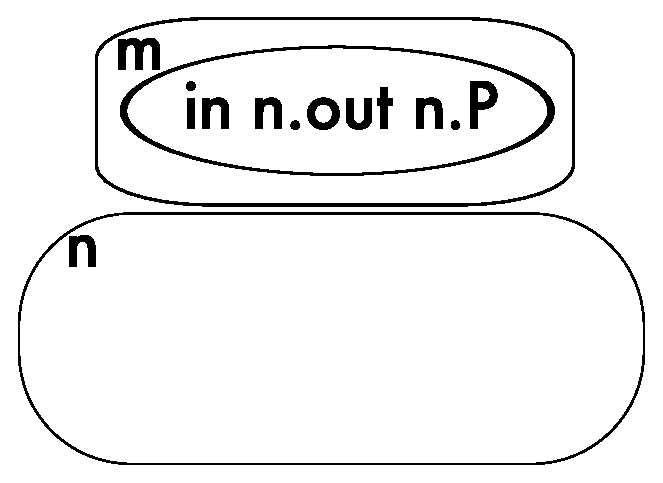
\includegraphics[scale=0.3]{ambient1}
  \caption{Spatial diagram of $m[\ambin{n}.\ambout{n}.P] \mid n[]$}
  \label{fig:ambient1}
\end{figure}

\begin{figure}  
  \centering
  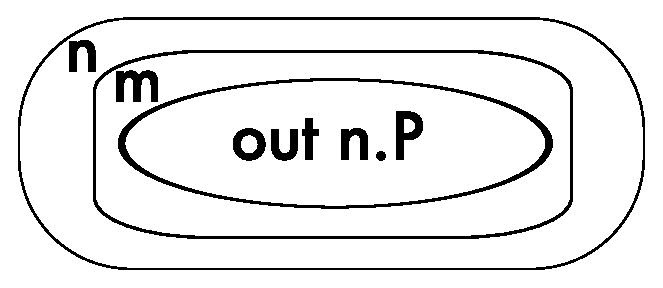
\includegraphics[scale=0.3]{ambient2}
  \caption{Spatial diagram of $n[m[\ambout{n}.P]]$}
  \label{fig:ambient2}
\end{figure}

\begin{figure}  
  \centering
  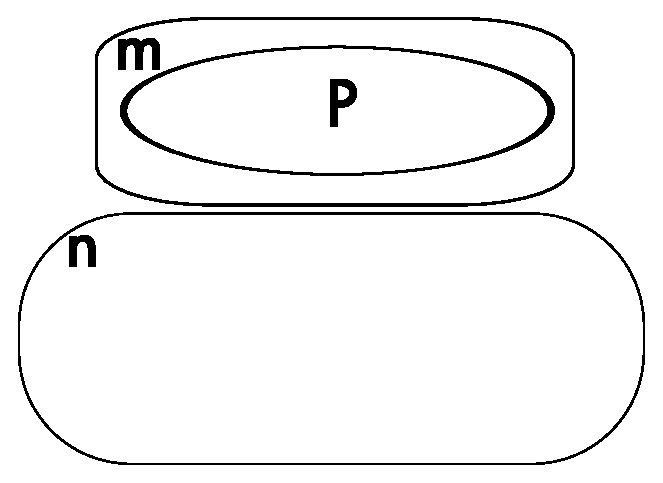
\includegraphics[scale=0.3]{ambient3}
  \caption{Spatial diagram of $m[P] \mid n[]$}
  \label{fig:ambient3}
\end{figure}

$open\ n$ is quite different.  It alters the structure, just as $in$ and
$out$ do, but rather than moving ambients, it destroys them.  It is also
applied to a child ambient rather than to the surrounding ambient, so
$open\ m.P\ |\ m[Q]$ (as in \cite{amb}) reduces to $P\ |\ Q$.

There are also issues with regard to the applicability of capabilities
and the use of the names.  A capability may only cause movement to occur
when at least one applicable ambient is available.  As such, movement
is heavily dependent on context, and specifically the availability of an
appropriately named ambient.  Applicability is dependent upon the
capability involved:

\begin{itemize}
\item For $\ambin{m}$, there must be a sibling of the surrounding
ambient named $m$.
\item For $\ambout{m}$, the parent of the surrounding ambient must be
named $m$.
\item For $\ambopen{m}$, there must be a child of the surrounding
  ambient named $m$.
\end{itemize}

All three capabilities are non-deterministic.  The same ambient name may
occur more than once, and each occurrence is regarded as being distinct.
As a result, the reduction of a capability includes a choice if there is
more than one applicable ambient present.  For example, $open\ m.P\ |\
m[Q]\ |\ m[R]$ has two possible derivations,

\begin{enumerate}
\item $open\ m.P\ |\ m[Q]\ |\ m[R] \rightarrow P\ |\ Q\ |\ m[R]$
\item $open\ m.P\ |\ m[Q]\ |\ m[R] \rightarrow P\ |\ m[Q]\ |\ R$
\end{enumerate}

The issue of non-determinism illustrates the behaviour that occurs when
there is more than one applicable ambient.  What about when there are
none?  The process stalls, and can not move on until such an ambient
becomes available.  This is akin to the situation in channel-based
calculi, such as CCS or the $\pi$ calculus, where a name is restricted,
but the appropriate co-name is not available to provide synchronisation.
For example,

\begin{equation}
(a.P) \backslash a 
\end{equation}

\noindent may never progress to become $P$ as there is no $\overline{a}$
for $a$ to synchronize with.  This behaviour is particularly relevant
with respect to $\ambout{m}$, where the sole use of the name is to stop
the surrounding ambient leaving its parent if the names don't match.

The restriction of ambient names, via $(\nu n) E$, combined with
mobility means that scope extrusion is also present in the calculus.
Just as the transmission of a name outside its scope causes extrusion
in the $\pi$ calculus, the restriction of ambient names may float
outward as necessary.  Scope intrusion is also possible in both
calculi, as demonstrated by the presence of the structural congruence
rule,

\begin{equation}
(\nu n)(P \pc Q) \equiv P \pc (\nu n) Q\ \text{if}\ n \not \in fn(P) \tag{Struct Res Par}
\end{equation}

\noindent which allows the restriction of $n$ to be removed from $P$
if the name doesn't occur free within its body.

\subsubsection{Variants of the Ambient Calculus}
\label{ambvariants}

A general problem within concurrency is the possibility of
\emph{interference}.  This was touched on briefly in the introduction
to this review, where the value of $x$ differed due to a race
condition.  In the ambient calculus, \emph{redex interference}
\cite{sangiorgi:mobsafeambients} is an issue, and is related to the
non-determinism mentioned above.

Take the example process from \cite{sangiorgi:mobsafeambients}.

\begin{equation}
n[\ambin{m}.P] \pc m[Q] \pc m[R]
\end{equation}

\noindent It is unclear what the environment of $P$ will be, following
the reduction of the capability, $\ambin{m}$.  There are two
alternatives,

\begin{enumerate}
\item $n[\ambin{m}.P] \pc m[Q] \pc m[R] \rightarrow m[n[P] \pc Q] \pc m[R]$
\item $n[\ambin{m}.P] \pc m[Q] \pc m[R] \rightarrow m[Q] \pc m[n[P] \pc [R]]$
\end{enumerate}

\noindent resulting from the two redexes formed between
$n[\ambin{m}.P]$ and $m[Q]$, and $n[\ambin{m}.P]$ and $m[R]$.  If one
contracts, resulting in a reduction, the other is no longer possible.
However, in this case, all three processes, $P$, $Q$ and $R$, can
still interact following either reduction.

In another example from the same paper,

\begin{equation}
\ambopen{n}.P \pc \ambopen{n}.Q \pc n[R]
\end{equation}

\noindent again with two possible interactions

\begin{enumerate}
\item $\ambopen{n}.P \pc \ambopen{n}.Q \pc n[R] \rightarrow P \pc \ambopen{n}.Q \pc R$
\item $\ambopen{n}.P \pc \ambopen{n}.Q \pc n[R] \rightarrow
  \ambopen{n}.P \pc Q \pc R$
\end{enumerate}


\noindent the resulting process includes a process, either $\ambopen{n}.Q$
or $\ambopen{n}.P$, which is stuck until such a time as another ambient
named $n$ appears as a parent.  This may never occur.  These kinds of
interference, referred to in \cite{sangiorgi:mobsafeambients} as
\emph{plain interferences}, may occur in other calculi.  The equivalent
in the $\pi$ calculus would be:

\begin{equation}
\overline{x}z.P \pc x(y).Q \pc x(y).R
\end{equation}

\noindent where again a reduction will occur between one of the two:

\begin{enumerate}
\item $\overline{x}z.P \pc x(y).Q \pc x(y).R \rightarrow P \pc Q\{z/y\}
  \pc x(y).R$
\item $\overline{x}z.P \pc x(y).Q \pc x(y).R \rightarrow P \pc x(y).Q
  \pc R\{z/y\}$
\end{enumerate}

\noindent and the remaining process, either $x(y).Q$ or $x(y).R$, will
be blocked.

Another more serious form of interference may occur in the ambient
calculus, due to the provision of differing interactions ($\ambin{m},
\ambout{m}$ and $\ambopen{m}$).  These \emph{grave interferences} occur
when an ambient is involved in two reductions occurring as the result
of different types of capability.  Take the example process,

\begin{equation}
\ambopen{n}.\nil \pc n[\ambin{m}.P] \pc m[Q]
\end{equation}

\noindent in which two reductions can occur that are logically
different.  While the interferences described above are a
representation of the kind of race conditions and non-determinism that
would be expected in any concurrent model, for example, to represent
competition for resources, grave interferences are usually unexpected
and typically represent errors in the model.  This process may perform
two radically different reductions,

\begin{enumerate}
\item $\ambopen{n}.\nil \pc n[\ambin{m}.P] \pc m[Q] \rightarrow \nil \pc
\ambin{m}.P \pc m[Q]$
\item $\ambopen{n}.\nil \pc n[\ambin{m}.P] \pc m[Q] \rightarrow
\ambopen{n}.\nil \pc m[n[P] \pc Q]$
\end{enumerate}

\noindent where either $n$ is destroyed, thus preventing the latter
movement of $P$ in to $m$ as it has no surrounding ambient, or $n$ moves
inside $m$ and is no longer available to be destroyed by
$\ambopen{n}.\nil$.  Clearly, only one of these reductions is likely to be
intentional.  

Levi and Sangiorgi's calculus of Mobile Safe Ambients \cite{safeamb00,
sangiorgi:mobsafeambients} presents a solution to this.  It introduces a
notion of co-capabilities, which enforce a pairing of mobility
primitives before a reduction can be made.  The result of this is that
the ambient being entered, exited or opened is aware of what is taking
place, and may react accordingly.

With these co-capabilities in place, the reduction rules for the
calculus run as follows:

\begin{align}
 n[\ambin{m}.P_1 \pc P_2] \pc m[\sambin{m}.Q_1 \pc Q2]
\rightarrow
m[n[P_1 \pc P_2] \pc Q_1 \pc Q_2] \tag{SafeIn}\\
 m[n[\ambout{m}.P_1 \pc P_2] \pc \sambout{m}.Q_2 \pc Q2]
\rightarrow
n[P_1 \pc P_2] \pc m[Q_1 \pc Q_2] \tag{SafeOut}\\
 \ambopen{n}.P \pc n[\sambopen{n}.Q_1 \pc Q_2]
\rightarrow
P \pc Q_1 \pc Q_2 \tag{SafeOpen} 
\end{align}

\noindent where, in each case, the capability must be able to
synchronize with a co-capability in the relevant ambient for the
reduction to take place.  For example, in SafeIn, $\ambin{m}.P_1$ must
pair up with $\sambin{m}.Q_1$ in the ambient $m$.  As a result, $Q_1$
can react appropriately to the change in structure, based on the fact
that it knows the movement has occurred.

The changes in the calculus of safe ambients, though simple, have a
dramatic effect on the ability to construct an algebraic theory for
the calculus and prove properties, especially when coupled with an
appropriate type system\footnote{In this case, the type system ensures
  single-threadedness, where only one process within an ambient may
  exercise a capability.}.  Essentially, they represent a move from
asynchronous to synchronous mobility primitives.  The calculus of
controlled ambients \cite{controlledamb02} restricts behaviour
further, by requiring that a co-capability must appear in both the
source and the destination.  Thus, an $\ambin{m}$ capability requires
permission both to leave its current location and to enter the
destination ambient. This is useful for the specific application of
the calculus, controlling resources, but is excessive in most
circumstances.

A further variant of the ambient calculus is the calculus of boxed
ambients \cite{boxedamb01}.  This removes the $open$ capability
altogether, replacing it with a form of directed communication inspired
by \cite{seal}.  Processes remain within their initial ambient
permanently (hence the term `boxed') and only the structure of the
ambient topology changes via the $in$ and $out$ capabilities.  Messages
may be sent locally, upwards or downwards, but not to siblings.

An example process from \cite{boxedamb01} is:

\begin{equation}
n[(x)^pP \pc p[\langle M \rangle \pc (x)Q \pc q[\langle N
\rangle^\uparrow ]]]
\end{equation}

\noindent where $n$, $p$ and $q$ are ambients, $(x)$ is an input and
$\langle M \rangle$ and $\langle N \rangle$ represent outputs.  $(x)Q$
may synchronize with either $\langle M \rangle$ locally or the upward
communication from $\langle N \rangle$.  $(x)^pP$ must synchronize with
$\langle M \rangle$, as the only output in $p$.

The ideas behind the boxed ambients calculus result in a formalism which
is more suited to communication-focused modelling, where the destruction
of locations would be unnatural.  Both it and the original ambient
calculus have their own particular niche, being suited to particular
applications.  In contrast, the latter is clearly more suited to
situations where the removal of a locality corresponds to a similar
event in the real-world situation being modelled.

\subsubsection{Advantages and Disadvantages of the Ambient Calculus}

The most interesting aspect of the ambient calculus is that, while it
includes no communication primitives, it can encode the asynchronous
$\pi$ calculus (see \ref{pivariants}).  This seems to imply that it is
possible to model mobility in a more natural way without losing much of
the expressivity of the $\pi$ calculus.  On consideration , this seems a
little less surprising as ambient names exhibit the same scope extrusion
seen with channel names in the $\pi$ calculus.  With this in mind, it is
not too difficult to see that ambient names could be used to mimic
channel names, with synchronisation being emulated by two processes
performing some kind of interaction within the same ambient.

However, the representation of synchronisation illustrated in \cite{amb}
seems to suggest that the ambient calculus may still have problems
dealing with the kind of global synchronisation needed for the
compositional broadcast agent considered in \ref{ccslimit}.  The
operation is performed by destroying and recreating ambients, as a
signal to the other process involved in the synchronisation.  Extending
this would seem to require using more ambients, which again leads to the
problem of enumerating the number of entities who wish to synchronize.
As before, this is possible but not compositional; every time
synchronisation is performed with a different number of agents, the
semantics of the process must be recreated.

Thus, the ambient calculus and the $\pi$ calculus have more in common
than is initially apparent, and the choice between the two seems to be
largely based on the most natural formalism for a particular task.

%\subsubsection{The Seal Calculus}

%The seal calculus \cite{seal}

\subsubsection{P Systems}
\label{psystems}

While providing a way of modelling concurrent spatially-oriented
systems, P Systems \cite{paun:98membranes} arise from the area of formal
language theory and re-writing rules rather than process
calculi.  They are considered here, as there exist a number of
similarities between them and, for example, the ambient calculus both in
providing a distributed model of computation and in finding applications
in the area of biological modelling.

A P system or \emph{transition super-cell system}
\cite{paun:98membranes} of degree $n$, where $n \ge 1$ is represented
as:

\begin{equation}
\Pi = (V, \mu, M_1, \dots, M_n,(R_1,\rho_1), \dots, (R_n,\rho_n),i_0)
\end{equation}

\noindent where:

\begin{itemize}
\item $V$ is an alphabet of objects.
\item $\mu$ is the membrane structure, containing $n$ membranes.
\item $M_i$, where $1 \le i \le n$, is a multiset of objects from $V$
      which are contained in membrane $i$.
\item $R_i$, where $1 \le i \le n$ is an evolution rule associated with
      one of the membranes, $i$. The corresponding $\rho_i$ is a
      partial-order relation which determines the priority of the rule.
      The rules are rewriting rules of the form $a \rightarrow v$, which
      causes $a$ to be replaced by $v$.
\item $i_0$ is a number between 1 and $n$ which specifies the \emph{output
      membrane} where the result of the computation should be found.
\end{itemize}

\noindent Any of the multisets, rules or priority relations may be
empty.  Evolution occurs in parallel, in a synchronous fashion involving
all membranes (referred to as \emph{maximal parallelism}).  A universal
clock is assumed to exist, which breaks the evolution of the system into
cycles.  Objects may move between membranes and membranes may be broken,
causing their objects to flood into the membrane above and their rules to
disappear.  Such behaviour has echoes of the ambient calculus described
in \ref{ambientcalculus}, where ambients may be destroyed by the $open$
primitive and processes may move around the ambient hierarchy (but only
within an ambient).  The notion of synchronous clock cycles also recalls
the discrete timed calculi of \ref{timing}, where evolution can also be
bounded by clock cycles in a synchronous fashion.  An interesting
distinction is commonly made in P systems; the outer membrane or
\emph{skin membrane} is assumed to be special.  For example, at least in
a biological context, the system is assumed to terminate if the outer
membrane is destroyed (biologically, the external membrane has been
broken and thus the organism falls apart).

Consider the following example P system (Fig. \ref{fig:psystem}),
\begin{align*}
\Pi_1 & = (V, \mu, M_1, M_2, M_3, M_4, (R_1, \rho_1), (R_2, \rho_2),
 (R_3, \rho_3), (R_4, \rho_4),4) \\
V & = \{a,b,b',c,f\} \\
\mu & = [_1[_2[_3]_3[_4]_4]_2]_1 \\
M_1 & = \emptyset, 
R_1 = \emptyset,
\rho_1 = \emptyset \\
M_2 & = \emptyset, 
R_2 = \{b' \rightarrow b, b \rightarrow b(c, in_4), r_1 : ff
 \rightarrow af, r_2 : f \rightarrow a\delta\},
\rho_2 = \{r_1 > r_2\} \\
M_3 & = \{af\},
R_3 = \{a \rightarrow ab', a \rightarrow b'\delta, f \rightarrow ff\},
\rho_3 = \emptyset \\
M_4 & = \emptyset,
R_4 = \emptyset,
\rho_4 = \emptyset
\end{align*}

\begin{figure}  
  \centering
  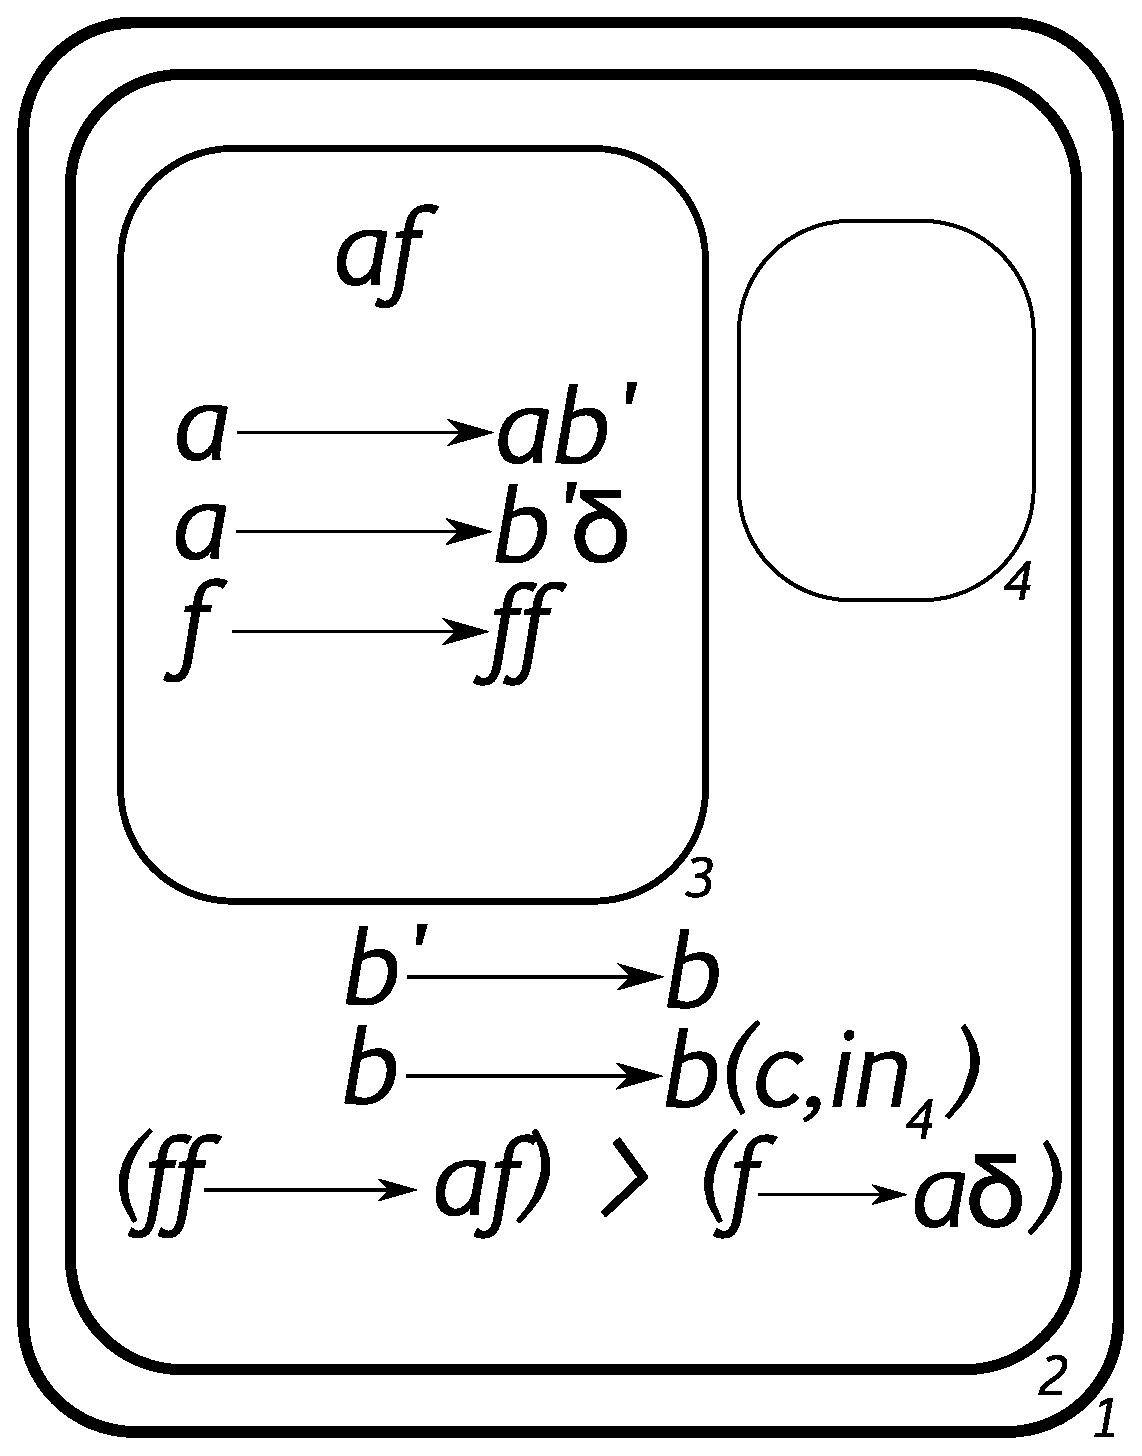
\includegraphics[scale=0.3]{psystem}
  \caption{Example P System}
  \label{fig:psystem}
\end{figure}

\noindent where the only membrane that initially contains any objects is
$M_3$.  In $M_3$ are two objects, $a$ and $f$.  $f$ only matches one
rule, $f \rightarrow ff$, which causes the number of $f$s to double on
each evolution.  For $a$, there are two rules and one is chosen
non-deterministically.  If the first, $a \rightarrow ab'$, is applied,
then an additional object $b'$ appears, and the rule may be applied
again as an $a$ is still present.  If $a \rightarrow ab'$ and $f
\rightarrow ff$ are applied for $n$ steps, then $n$ instances of $b'$
and $2^n$ occurrences of $f$ are present.

If the second $a$ rule $a \rightarrow b'\delta$, is applied, the
$\delta$ causes the membrane, $M_3$, to be dissolved.  At this point,
there will be one extra $b'$ and one extra $f$ resulting from the
application of this rule and $f \rightarrow ff$, respectively, and no
$a$.  This changes the configuration of the system to become:
\begin{align*}
\mu & = [_1[_2[_4]_4]_2]_1 \\
M_1 & = \emptyset, 
R_1 = \emptyset,
\rho_1 = \emptyset \\
M_2 & = \{b'^{n+1}, f^{2n+1}\} \\ 
R_2 & = \{b' \rightarrow b, b \rightarrow b(c, in_4), r_1 : ff
 \rightarrow af, r_2 : f \rightarrow a\delta\},
\rho_2 = \{r_1 > r_2\} \\
M_4 & = \emptyset,
R_4 = \emptyset,
\rho_4 = \emptyset
\end{align*}

\noindent The three rules that were present in $M_3$ are lost, while the
objects float into the membrane above, $M_2$.  In this configuration,
$n$ represents the number of times the pair of rules $a \rightarrow ab'$
and $f \rightarrow ff$ were applied prior to this, and is greater than
or equal to zero.

In $M_2$, a priority relation exists that forces $ff \rightarrow af$ to
be given precedence over $f \rightarrow a\delta$.  As a result, whenever
it is possible to apply $ff \rightarrow af$ (i.e. there are two $f$
objects), it will be applied instead of $f \rightarrow a\delta$.  The
other two rules manipulate the $b'$ objects. First, they are all
converted in to $b$ objects.  This will always occur, as there are at
least two $f$ objects in $M_2$ to begin with, which means $ff
\rightarrow af$ will be applied rather than $f \rightarrow a\delta$
which destroys $M_2$.  Each time $ff \rightarrow af$ is applied, the
number of $f$ objects halves.

The remaining rule, $b \rightarrow b(c, in_4)$, will evolve once for
each occurrence of $ff$, of which there are $n$.  $M_2$ contains $n + 1$
$b$ objects, all converted from the $b'$ objects that were in $M_3$.  As
long as there is an even number of $f$ objects, the two rules $b
\rightarrow b(c, in_4)$ and $ff \rightarrow af$ will be applied, halving
the number of $f$ objects and creating $n + 1$ c objects in $M_4$ (via
$(c, in_4)$), while the number of $b$ objects remains the same.

When only one $f$ object is left, $f \rightarrow a\delta$ will be
applied, resulting in $M_2$ being destroyed and the following
configuration:
\begin{align*}
\mu & = [_1[_4]_4]_1 \\
M_1 & = \{a^{2n+1},b^{n+1}\}, 
R_1 = \emptyset,
\rho_1 = \emptyset \\
M_4 & = \{c^{(n+1)^2}\},
R_4 = \emptyset,
\rho_4 = \emptyset
\end{align*}

\noindent No further evolution is possible, as there are no more rules.
$c^{(n+1)^2}$ is the final output, as $M_4$ is the output membrane.

Further variants of P systems exist.  Tissue P systems use a graph-based
structure rather than the tree shown here, while population P systems
also incorporate an environment.  At present, the main flaw with
modelling concurrent systems using this formalism is that the underlying
theory is not as advanced as for those of process calculi,
such as the $\pi$ calculus.  So far, P systems research has focused on
their power of expressivity, and their application within the field of
biological modelling.  In the latter, they provide a much more natural
perspective than the channel-based operations of the $\pi$ calculus, and
this is something that will be considered further in section \ref{bioapps}.

\subsubsection{Bigraphs}
\label{bigraphs}

Bigraphs \cite{bigraph1, bigraph2} are an attempt at providing a
unifying framework, able to represent both spatial relationships
(\emph{locality}) in the style of the ambient calculus (see
\ref{ambientcalculus}) and link-based-relationships
(\emph{connectivity}) seen in the $\pi$ calculus (see \ref{picalculus}).
Their particular application area is within pervasive computing, where a
mixture of both concepts is needed to represent both movement through
space and the change in relationships between agents.

The nodes in a bigraph support a dual structure, hence the name.  On one
level, there are nodes nested within nodes, representing locality.  This
is called the \emph{place graph}.  These nodes have \emph{ports} which
are connected via links to form a \emph{link graph}.  Each node has a
\emph{control} with an arity that defines the number of ports.  The two
graphs share nodes, but are otherwise independent.  Nesting can only
occur in nodes with a \emph{non-atomic} control.  These can also be
\emph{active} or \emph{passive}.  The former allows reactions to occur
within the node.  \emph{Holes} may occur in bigraphs, where other
bigraphs can appear.

Within this model, it is possible to encode both the $\pi$ calculus and
the ambient calculus.  Take the following rule from the asynchronous
$\pi$ calculus without summation,

\begin{equation}
\overline{x}y \pc x(z).P \rightarrow P\{y/z\}
\end{equation}

\noindent which represents synchronisation.  In \cite{bigraph1}, Milner
encodes this as a bigraph with two controls, $send$ and $get$, both of
which have an arity of two.  To represent the fact that the output
prefix has no continuation in the asynchronous $\pi$ calculus, $send$ is
declared atomic.  $get$ is non-atomic but inactive.

The node $get$ includes a nested hole with the port $z$.  This
represents the continuation $P$, with $z$ being the name bound on
input.  The port $z$ is linked from the hole to $get$ itself.  $send$
has two ports: $x$, which is also connected to $get$, and $y$.  With
these concepts in place, the reaction may be represented as:

\begin{equation}
send_{xy} \pc get_{x(z)} \square \rightarrow x \pc y/(z) \square
\end{equation}

\noindent the $send$ node disappearing afterwards, leaving $y$ connected
to $z$ and $x$ unused.

Similarly, \cite{bigraph1} shows how the $in$ capability from the
ambient calculus:

\begin{equation}
 n[\ambin{m}.P_1 \pc P_2] \pc m[Q]
  \rightarrow
  m[n[P_1 \pc P_2] \pc Q] \\
\end{equation}

\noindent may be encoded using two controls, $amb$ and $in$, both with
an arity of one.  The two ambients involved are represented by
instances of $amb$, while $in$ is an atomic control representing the
process that emits the capability.  The $amb$ control is non-atomic
and active, each ambient containing a hole which represents their
continued behaviour,

The ambient names are represented as the node's single port.  In the
case of the ambient named in the capability, this is also linked to the
$in$ instance.  To model the reaction above, $n$ is connected to the
port of one $amb$, while $m$ is connected to both the other $amb$ and
$in$.  The reaction is then encoded as:

\begin{equation}
amb_n (in_m \pc \square_0) \pc amb_m \square_1
\rightarrow
amb_m (amb_n \square_0 \pc \square_1)
\end{equation}

\noindent where the similarities between the two are clear.

Bigraphs provide an interesting framework for unifying the two disparate
concepts outlined above in \ref{scopemobility} and \ref{migration}.  It
will be exciting to see how this theory develops, and whether it can
also be used to encode the discrete time notions described in \ref{timing}.

\section{Typed Calculi}
\label{typedcalculi}

A common addition to a process calculus is a type system, especially
in recent literature which attempts to use such calculi as the basis
for a programming language or a distributed system.  Type systems can
be used to restrict the calculus in ways that aren't always possible
via mere manipulation of the syntax and semantics.  Adding a type
system can be as simple as formalising implicit notions, such as the
use of $\ambin{m}$ as a capability and not as part of a path
\cite{ambienttypes} or the fact that the $x$ in $x(y)$ should be
represent a link and not a mere value \cite{sangiorgi:types-or}.  It
may also provide more complex intuitions, by distinguishing individual
entities, controlling mobility \cite{sangiorgi:mobsafeambients,
  ambienttypes} or resources \cite{hennessy:dpi98} or even providing a
full subtyping relation \cite{sangiorgi:typing, boxedamb02}.  This
section considers a few examples of such type systems for both the
$\pi$ calculus (\ref{pitypes}) and the ambient calculus
(\ref{ambienttypes}).

\subsection{Type Systems for the $\pi$ Calculus}
\label{pitypes}

Various type systems have been introduced for the $\pi$ calculus in
the literature, ranging from the simple notion of sorts introduced by
Milner \cite{milner:pi} to those introduced for a specific purpose
\cite{sangiorgi:types-or} and more complex systems involving subtyping
\cite{sangiorgi:typing}.  Here, sorts are considered followed by a
brief look at the distinction between values and links made by
Sangiorgi \cite{sangiorgi:types-or} for the purpose of proving
termination.

\subsubsection{Sorts}

The earliest notion of types was introduced by Milner in
\cite{milner:93polyadic, milner:pi}.  The discipline of \emph{sorts}
is simply a way of representing `the length and nature of the vector
of names a name may carry in communication' \cite{milner:93polyadic}.
Formally, a sort is a partial function,

\begin{equation}
ob : \Sigma \rightarrow \Sigma^*
\end{equation}

\noindent mapping a name to a vector of names.  From this, it is
simple to define a sort for all communications in CCS and CaSE as
$\{NAME \mapsto ()\}$ (as nothing is passed) and the monadic $\pi$
calculus as $\{NAME \mapsto (NAME)\}$.

Take the simple example of a buffer,

\begin{equation}
  Buf \eqdef (in,out)(in(x).\overline{out}x.Buf\langle in,
  out\rangle 
\end{equation}

\noindent which simply receives a value on $in$ and transmits it on
$out$.  $x$ may be assigned the sort $s_1 \mapsto S$, where $S$ is the
unknown sort of the buffered value and $s_1$ is an arbitrary name for
the new sort.  From this, it follows that both the $in$ and $out$
channels have the sort $s_2 \mapsto (s_1)$, as they both receive or
transmit $x$.

The purpose behind introducing sorts is to make explicit the need to
match the number of values being received with the number being sent.
Matching the length of these vectors becomes a necessity when dealing
with the polyadic $\pi$ calculus, which doesn't have the same uniform
sort for all channels as is present in CCS, CaSE or the $\pi$
calculus.

Consider the example from \cite{milner:pi} of two processes, $P$ and
$Q$:

\begin{align}
P & \eqdef x(y).\overline{y}uv.\nil \\
Q & \eqdef \overline{x}y'.y'(w).Q' 
\end{align}

\noindent where the parallel composition of these two processes should
be disallowed.  This is made clear following the first reduction that
would result from such a composition:

\begin{equation}
P \pc Q \rightarrow \overline{y'}uv.\nil \pc y'(w).Q'
\end{equation}

\noindent where $Q$ transmits $y'$ to $P$.  $P$ then tries to use $y'$
to transmit two values, $u$ and $v$, whereas $y'$ is only used with
one, $w$, in the input of $Q$.  Applying an appropriate sort discipline,

\begin{equation}
\begin{aligned}
u: s_1 & \mapsto S \\
v: s_2 & \mapsto T \\
w: s_3 & \mapsto (s_1) \\
y: s_4 & \mapsto (s_1, s_2) \\
y': s_5 & \mapsto (s_1)
\end{aligned}
\end{equation}

\noindent allows the typing of $x$ to be prevented by distinguishing
between types based on the length of the sort.  In $P$, $x$ must have
a sort of length two, while in $Q$, its sort would only be of length
one.  This kind of type system formalises an intuition already adopted
implicitly (that the length of the input vector should equal that of
the output vector), which is a common methodology for type systems.

\subsubsection{Typing for Termination}

A similar realisation of implicit assumptions is made by Sangiorgi
\cite{sangiorgi:types-or} and is used to prove termination for a
subset of possible $\pi$ calculus processes.  The type system is used
to explicitly realise the \emph{order} of a name.  The types use the
simple grammar,

\begin{equation}
T ::= \#T \pc unit
\end{equation}

\noindent where $unit$ represents a value and a series of $\#$ symbols
is used to represent the level of indirection which exists between the
value and the current name.  For example, $\#unit$ is the type of a
\emph{first-order link}, representing a name which is used to pass
values between processes.  A type with more than one $\#$ represents a
\emph{higher-order link}, which is used to pass links between
processes.

This notion is used within the fragment of the type system shown in
Table \ref{tab:sangrules} to restrict the possible types used in input
and output prefixing, and restriction.  The rule T-Out ensures
that an output prefix, $\overline{v}w.M$, is only typeable if:

\begin{table}
  \caption{Typing Rules from \cite{sangiorgi:types-or}}
  \label{tab:sangrules}
  \shrule
 \begin{center}
 \begin{tabular}{c}
     \Rule{\sc{T-Out}\ \ }
     {\vdash v : \#T, \vdash w : T, \vdash M}
     {\vdash \overline{v}w.M}
     {}
  \\[3ex]
  \Rule{\sc{T-Inp}\ }
     {\vdash v : \#T, x \in T, \vdash M}
     {\vdash v(x).M}
     {}
  \\[3ex]
     \Rule{\sc{T-Res}\ \ }
     {x_i \in \#T_i\ \text{for some}\ T_i (1 \le i \le n), \vdash M}
     {\vdash (x_1 \dots x_n) M}
     {}
 \end{tabular}
  \end{center}
  \shrule
\end{table}

\begin{itemize}
\item $v$ is at least a first-order link (it has one or more $\#$s)
\item $w$ has a type, $T$
\item The continuation, $M$, is typeable
\end{itemize}

\noindent which prevents $v$ from being a simple value.  Similarly,
T-In restricts $v$ to being at least a first-order link in
$v(x).M$ and T-Res ensures that each restricted name is a link.

These are all ideas that are adopted implicitly in using the $\pi$
calculus to model systems, but, when not enforced by a type system,
these properties can not be included in proofs.  The type system in
Sangiorgi's paper, although simple, allows a set of processes which
are syntactically correct, but logically flawed, to be excluded by
only considering processes which are typeable.

%\subsubsection{The Type System of the Distributed $\pi$ Calculus}

\subsection{Type Systems for the Ambient Calculus}
\label{ambienttypes}

Early work \cite{commtypesamb} on providing a type system for the
ambient calculus focused on typing the derived communication primitives
and specifically the values being exchanged.  While interesting, this
doesn't really relate to the focus of the calculus, spatial mobility.
In \cite{cardelli:typesforambients, cardelli:ambienttypes}, a first
attempt is made at providing types for mobility, via mobility and locking
annotations.  Mobility annotations are used to mark an ambient as mobile
($\underline{\vee}$) or immobile ($\curvearrowright$), where mobile
ambients may be involved in movement operations using the capabilities
$in$ and $out$.  Locking annotations control the use of $open$; locked
ambients ($\bullet$) may not be the target of an $open$ capability,
while unlocked ambients ($\circ$) may.

A more general theory is given in \cite{ambienttypes} with the
introduction of \emph{groups}.  Rather than simply specifying whether or
not an ambient can move or be destroyed, the type system is more
specific as to which ambients may effect others.  To avoid dependent
types \cite{deptypes}, where the types are dependent on the values being
typed, an intermediary notion of a group is introduced.  This is also
advantageous in that it allows a series of ambients to have the same
typing, while typing in relation to a single ambient is still possible
by having a group with only one member.

For example, given two ambients $m$ and $n$, the types should express
that $n$ can enter $m$.  A dependent formalisation would say that $n$
has the type $CanEnter(m)$, while, using groups, $m$ is given the type
$G$ (where $G$ is a group) and $n$ is typed as $CanEnter(G)$.  Within
the type system itself, ambients are allocated to groups via the use of
a group binder, $(\nu G)$.  Just like the ambient binder, $(\nu n)$,
the scope of this may extrude outwards.  However, the type system
prevents it from ever encapsulating ambients which did not form part of
its initial scope (i.e. it only tracks the movements of ambients that
are a member of that group).  Within the paper, groups are used to
assign properties to its members, such as the type of communication
possible and the control of crossing or opening ambients.

The types of messages or \emph{exchanges} may specify either no
communication ($Shh$) or a tuple of partners for the communication:

\begin{equation}
S, T ::= Shh \pc W_1 \times \dots \times W_k
\end{equation}

\noindent For example, in the simplest form of the calculus,
$Agent[Shh]$ represents a group called $Agent$, the members of which may
not exchange values.  Nesting is possible, so $Place[Agent[Shh]]]$
represents a $Place$ where groups of $Agent$s may stay and continue to
be silent.

The full type system, given in \cite{ambienttypes}, includes these
exchange types along with types to control the opening and crossing of
ambients.  Groups are parameterised over $F$,

\begin{equation}
F ::= ^\curvearrowright \mathbf{G}, ^\circ \mathbf{H}, T
\end{equation}

\noindent with the final form of ambient type being $G^\curvearrowright
\mathbf{G'}[F]$.  $\mathbf{G'}$ represents the groups that the ambient
may cross via objective moves (introduced in the same paper), while
$\mathbf{G}$ includes the groups that the ambient may cross via standard
subjective movement.  Finally, $\mathbf{H}$ distinguishes the groups
whose ambients may be $\ambopen{e}$, while $T$ is as defined above.

A similar system is adopted in \cite{m3}, but, as this refers to boxed
ambients (see \ref{ambvariants}), no control of $open$ is required.  It
does introduce a new set of groups, however, to handle the lightweight
process mobility presented.  In both cases, the type system has a
positive effect on the calculus.  Not only does it alleviate some of
the syntax ambiguity, but it also allows a more fine-grained notion of
mobility, where specific ambients can be made immobile or unable to
cross a particular ambient.

\section{Biological Applications}
\label{bioapps}

Biological systems are inherently concurrent, being focused on the
behaviour of multiple entities from low-level molecules, through
bacteria and other bodies, to full cellular structures and beyond.
Models which incorporate spatial distribution, such as the ambient
calculus (\ref{ambientcalculus}) and P systems (\ref{psystems}) are
especially useful for representing the structure of real-world
biological entities.

Such modelling is becoming common place within the
literature\cite{biospi, cardelli:bioambients, fran}, where concurrent
models represent an alternative to the use of ordinary differential
equations (ODEs).  The usual approach is to create a model of the
system within the formalism and then perform simulations.  Such
simulations rely on reducing the non-determinism within the model by
introducing a stochastic semantics.  In each of the biochemical
stochastic $\pi$ calculus \cite{biospi}, the BioAmbient variant
\cite{cardelli:bioambients} and P systems \cite{fran}, these are based
on Gillespie's algorithm \cite{gillespie}.

The algorithm selects which reaction occurs next and the necessary
advancement of the system's `clock' (a real time value in this context,
rather than some discrete notion).  A probability is associated with
each reaction, so that the algorithm basically runs as follows:

\begin{enumerate}
\item $a_0$ is calculated as the sum of the probabilities.
\item Two random numbers, $r_1$ and $r_2$, are generated from a uniform
      distribution over the unit interval 0 to 1.
\item Calculate the waiting time for the next reaction, $\tau_i =
      \frac{1}{a_0} \ln (\frac{1}{r_1})$
\item Take the index, $j$, of the reaction such that
      $\displaystyle\sum_{k=1}^{j-1} p_k < r_2 a_0 \le
      \displaystyle\sum_{k=1}^jp_k$ where $p_k$ is the $k$th probability.
\item Return the pair $(\tau_i, j)$
\end{enumerate}

\noindent determining which one occurs.  Slight alterations are made in
distributed models to handle the rules arising from different localities.
For example, the P systems model \cite{fran} adapts the algorithm to
form a multi-compartmental variant, which treats each membrane
separately, to a degree, while also taking into account that activity
in one membrane may affect others.

Clearly, different formalisms offer different approaches.  In the
original $\pi$ calculus approach of \cite{biospi}, the focus was solely
on communication with biological compartments abstracted as private
channels.  The model given for BioAmbients \cite{cardelli:bioambients}
is more natural due to the explicit realisation of these compartments.

Take the following example from \cite{cardelli:bioambients},

\begin{equation}
\begin{aligned}
\mathtt{System} & ::= \mathtt{molecule[Mol] \pc \dots \pc molecule[Mol] \pc
 cell[Porin]} \\
\mathtt{Mol} & ::= \mathtt{enter\ cell1.Mol + exit\ cell2 . Mol} \\
\mathtt{Porin} & ::= \mathtt{accept\ cell1.Porin + expel\ cell2.Porin}
\end{aligned}
\end{equation}

\noindent which demonstrates a membranal pore, which molecules use to
pass through a membrane.  Both the cell and the molecules are
represented by ambients.  Each molecule is controlled by a process,
$Mol$, which, at any time, has the option of performing either an
\texttt{enter} or an \texttt{exit}.  Similarly, the $Porin$ process,
which represents the membranal pore, may \texttt{accept} or
\texttt{expel}.

Within the BioAmbient calculus, movement is synchronous and takes place
by the pairing of an \texttt{enter} and \texttt{accept} action (the
equivalent of $in$) or an \texttt{exit} and \texttt{expel} action
(equivalent to $out$).  The first action in each case is used by the
moving process.  Both must also mention the same channel name
(\texttt{cell1} and \texttt{cell2} here).  In the case of the system
shown above, both \texttt{Mol} and \texttt{Porin} permanently offer
their halves of this pairing.  However, the spatial context makes one of
them inapplicable.  Initially, \texttt{exit} and \texttt{expel} won't
synchronize, as \texttt{Mol} is not inside the ambient from which it is
being expelled.  Likewise, once it has entered, it can't do so again,
even though the actions make this possible.

Models such as this seem a little unnatural as molecules are modelled as
both an ambient and a process.  This is because only ambients may move
but only processes can emit the necessary mobility primitives to do so.
The notions of mobility present in the ambient calculus, including this
idea, have been carried across, even though it doesn't directly adopt
the primitives of the ambient calculus; the style is still more akin to
the $\pi$ calculus.

In contrast, \cite{fran} takes a different approach using P systems,
representing signals and proteins directly as objects in the membranes.
One particular application of this technique is \emph{quorum sensing}.
This is a gene regulation system where a population of bacterial cells
communicate in order to regulate the expression of certain genes in a
co-ordinated way which is dependent on the size of the population.
\cite{fran} presents a model of this phenomenon in \emph{vibrio
fischeri}, a marine bacterium, using a P system\footnote{This method of
defining the configuration differs slightly from that in \ref{psystems},
as it also includes a set of labels, rather than assuming that the
natural numbers are used.}:
\begin{align*}
  \Pi_{vf} & = (O, \{e,b\}, \mu, (w_1, e), (w_2, b), \dots,
  (w_{n+1},b),\mathcal{R}_b, \mathcal{R}_e) \\
  O & = \{OHHL, LuxR, LuxR\text{-}OHHL, LuxBox, LuxBox\text{-}LuxR\text{-}OHHL\} \\
  w_1 & = \emptyset \\
  w_i & = \{LuxBox\}\ \text{where}\ 2 \le i \le n + 1 \\
\end{align*}

\noindent where each bacteria is represented as a membrane, $b$, within
an environment membrane, $e$.  The alphabet, $O$, contains the signal,
$OHHL$, the protein, $LuxR$ and the regulatory region, $LuxBox$, in
addition to the protein-signal complex ($LuxR-OHHL$) formed and its
regulatory region, $LuxBox-LuxR-OHHL$.  The initial configuration shown
above leaves the environment empty and places just the genome, $LuxBox$,
inside each bacteria membrane to start production of the signal and the
protein.  $\mathcal{R}_b$ and $\mathcal{R}_e$ contain the rules which
affect the bacteria and the environment respectively.  The reader is
referred to the full paper for full details of these.

This model seems much more natural and has a clearer correspondence with
the real-world representation.  The main issue, as noted earlier in
\ref{psystems}, is that the theory of P systems is not as well developed
as that of the $\pi$ calculus (upon which the BioAmbients calculus is
essentially based).  This can prove problematic, especially when model
checking such models.

\section{Conclusion}

In conclusion, this review has taken a brief look at the field of
concurrency, largely from the perspective of process calculi.
Initially, it was shown that, while universal Turing machines and the
$\lambda$ calculus can simulate any recursive function, their inherent
sequential behaviour makes them unsuitable for modelling concurrent
systems.  CCS, in contrast, is less expressive but can model this kind
of behaviour.

The $\pi$ calculus seems to provide the best of both worlds, being able
to model concurrent systems and still retain the expressiveness of the
$\lambda$ calculus.  However, a key limitation was identified which
reinforced the idea that expressivity only makes a model capable, and
not suitable, for simulating any recursive function: modelling global
synchronisation via a broadcasting agent.  This limitation seems to hold
for both CCS and the $\pi$ calculus, and it is also likely that it
applies to many other process calculi, such as the ambient calculus, a
formalism that provides a more natural form of mobility via structural
changes.

Discrete timed calculi can overcome this.  An example using TPL to
model a compositional broadcasting agent, using semantics suitable for
any arbitrary number of processes, is provided in \ref{timing}.
Extensions to TPL, such as CaSE, may scale even further using
synchronous encapsulation to create systems of multiple components.

Type systems were also briefly considered as a way of restricting the
behaviour of a process algebraic model.  These tend to explicitly reduce
the expressivity of the formalism in order to ensure that unwanted
constructs can not be created by making them untypeable.  This also
makes it easier to prove properties of the calculus.  Biology was also
considered briefly (see \ref{bioapps}), as a potential application area.
P systems seem the most natural formalism, but they lack some of the
proven theoretical aspects of process calculi.

Following much consideration of the available literature, the concept of
a calculus which combines both the mobility of the $\pi$ and ambient
calculi with the inherent scalability of a calculus like CaSE seems
novel.  This research hopes to provide just such a formalism.



